\documentclass{article}

\pdfoutput=1

% if you need to pass options to natbib, use, e.g.:
\PassOptionsToPackage{numbers, compress}{natbib}
% before loading nips_2016
%
% to avoid loading the natbib package, add option nonatbib:
% \usepackage[nonatbib]{nips_2016}

\usepackage[final]{nips_2016}

% to compile a camera-ready version, add the [final] option, e.g.:
% \usepackage[final]{nips_2016}

\usepackage[utf8]{inputenc} % allow utf-8 input
\usepackage[T1]{fontenc}    % use 8-bit T1 fonts
\usepackage{hyperref}       % hyperlinks
\usepackage{url}            % simple URL typesetting
\usepackage{booktabs}       % professional-quality tables
\usepackage{amsfonts}       % blackboard math symbols
\usepackage{nicefrac}       % compact symbols for 1/2, etc.
\usepackage{microtype}      % microtypography

\usepackage{floatrow}       % set figure and table side-by-side

% For math and shiz
\usepackage{amsmath}
% For writing lemmas and proofs.
\usepackage{amsthm}
\usepackage{amssymb}
% For less list spacing
\usepackage{enumitem}
% For math and shiz
\usepackage{mathtools}
% use Times
\usepackage{times}
% For figures
\usepackage{graphicx} % more modern
%\usepackage{epsfig} % less modern
\usepackage{subcaption}
% Stack anchor
\usepackage{stackengine}

\usepackage{siunitx}
\usepackage{lscape}

% For citations
%\usepackage{natbib}

% For algorithms
\usepackage{algorithm}
\usepackage{algorithmic}

% As of 2011, we use the hyperref package to produce hyperlinks in the
% resulting PDF.  If this breaks your system, please commend out the
% following usepackage line and replace \usepackage{icml2016} with
% \usepackage[nohyperref]{icml2016} above.
\usepackage{hyperref}


% Packages hyperref and algorithmic misbehave sometimes.  We can fix
% this with the following command.
%\newcommand{\theHalgorithm}{\arabic{algorithm}}
\newcommand{\K}{\!\{\!K\!\}}
\newcommand{\KL}{\!\{\!K_L\!\}}
\newcommand{\W}{\scriptscriptstyle W}
\newfloatcommand{capbtabbox}{table}[][\FBwidth]

% Theorem
\newtheorem{theorem}{Theorem}
\newtheorem{lemma}{Lemma}
\newtheorem{definition}{Definition}

\title{Scaling Memory-Augmented Neural Networks with Sparse Reads and Writes}

% The \author macro works with any number of authors. There are two
% commands used to separate the names and addresses of multiple
% authors: \And and \AND.
%
% Using \And between authors leaves it to LaTeX to determine where to
% break the lines. Using \AND forces a line break at that point. So,
% if LaTeX puts 3 of 4 authors names on the first line, and the last
% on the second line, try using \AND instead of \And before the third
% author name.


\author{
% TODO fight with the NIPS template for the over the author-list (doesn't matter for the original submission).
%\icmlauthor{Jack W Rae}{jwrae@google.com}
%\icmladdress{Google DeepMind,}
%\icmlauthor{Jonathan J Hunt}{jjhunt@google.com}
%\icmladdress{Google DeepMind}
%\icmlauthor{Ivo Danihelka}{danihelka@google.com}
%\icmladdress{Google DeepMind}
%\icmlauthor{Tim Harley}{tharley@google.com}
%\icmladdress{Google DeepMind}
%\icmlauthor{Andrew Senior}{andrewsenior@google.com}
%\icmladdress{Google DeepMind}
%\icmlauthor{Greg Wayne}{gregwayne@google.com}
%\icmladdress{Google DeepMind}
%\icmlauthor{Alex Graves}{gravesa@google.com}
%\icmladdress{Google DeepMind}
%\icmlauthor{Timothy P Lillicrap}{countzero@google.com}
%\icmladdress{Google DeepMind}
Jack W Rae\footnotemark[1] \\
\texttt{jwrae}
\And
Jonathan J Hunt\footnotemark[1] \\
\texttt{jjhunt}
\And
Tim Harley\\
\texttt{tharley}
\And
Ivo Danihelka \\
\texttt{danihelka}
\And
Andrew Senior \\
\texttt{andrewsenior}
\And
Greg Wayne \\
\texttt{gregwayne}
\And
Alex Graves \\
\texttt{gravesa}
\And
Timothy P Lillicrap \\
%\textt{countzero}
\texttt{countzero}
\\
\\
\hspace{-8.3cm}
Google DeepMind \\
\hspace{-8.3cm}
\texttt{@google.com}
  %% examples of more authors
  %% \And
  %% Coauthor \\
  %% Affiliation \\
  %% Address \\
  %% \texttt{email} \\
  %% \AND
  %% Coauthor \\
  %% Affiliation \\
  %% Address \\
  %% \texttt{email} \\
  %% \And
  %% Coauthor \\
  %% Affiliation \\
  %% Address \\
  %% \texttt{email} \\
  %% \And
  %% Coauthor \\
  %% Affiliation \\
  %% Address \\
  %% \texttt{email} \\
}

\begin{document}
% \nipsfinalcopy is no longer used

\maketitle

\renewcommand{\thefootnote}{\fnsymbol{footnote}}
\footnotetext[1]{These authors contributed equally.}

% TODO add appendix on the SDNC.

\begin{abstract}
Neural networks augmented with external memory have the ability to learn algorithmic solutions to complex tasks. These models appear promising for applications such as language modeling and machine translation. However, they scale poorly in both space and time as the amount of memory grows --- limiting their applicability to real-world domains. Here, we present an end-to-end differentiable memory access scheme, which we call Sparse Access Memory (SAM), that retains the representational power of the original approaches whilst training efficiently with very large memories. We show that SAM achieves asymptotic lower bounds in space and time complexity, and find that an implementation runs $1,\!000\times$ faster and with $3,\!000\times$ less physical memory than non-sparse models. SAM learns with comparable data efficiency to existing models on a range of synthetic tasks and one-shot Omniglot character recognition, and can scale to tasks requiring $100,\!000$s of time steps and memories. As well, we show how our approach can be adapted for models that maintain temporal associations between memories, as with the recently introduced Differentiable Neural Computer.


%for the Differentiable Neural Computer (DNC) architecture, a recently published memory which
%model which maintains is more adaptable than previous memory models. Our sparse DNC maintains the speed advantages of SAM, while incorporating the temporal association mechanisms in the DNC.

%Finally, we demonstrate SAM is able to learn character recognition in one-shot when trained on the ``omniglot'' dataset, with competitive data efficiency to existing dense models.
% TODO (maybe update this final sentence when we decide what is going in the paper.
%TODO decide upon this last sentence.
%We do this by limiting memory updates to a small number of contextually relevant rows in the external memory.
%We show that it can be trained in $\Theta(1)$ space and $\Theta(\log N)$ time per step, where $N$ is the number of words stored in memory.
\end{abstract}


\section{Introduction}
%Recurrent neural networks, trained using backpropagation through time \cite{werbos1990backpropagation}, are powerful models for sequence learning.
%Unlike hidden Markov models, the representational capacity of neural networks grows exponentially with the size of the hidden state.
%In particular, Long Short-Term Memory or LSTM \cite{hochreiter1997long},
%which addresses the ``vanishing or exploding gradients'' problem, is now widely used to solve
%many sequential tasks \cite{graves2013speech, sutskever2014}. % TODO add some more references here
%One limitation of these models is that the number of parameters and computational cost grows proportionally to the square of the size of the recurrent state.

%More recently, there have been some notable successes with models which use large ``external'' memories accessed by a much smaller controller module
%\cite{graves2014neural,weston2014memory,bahdanau2014neural,zaremba2015reinforcement, vinyals2015pointer}. The controller is a neural network that instructs the reading and writing of words to memory. One exemplar is the Neural Turing machine (NTM) \cite{graves2014neural}, which incorporates read and write heads to access the external memory in a fully differentiable manner.
%%uses an ``external''
%%content-addressable memory. In analogy with the Turing machine, this large external memory can be read and written by a controller network.
%%The read and write operations are ``soft'' rather than discrete as in a conventional computer, allowing the entire system to be differentiable.
%The NTM is capable of learning algorithmic solutions to problems that, unlike the LSTM, generalize to much longer sequences than seen during training. %As discussed later, there have been a number of other related and interesting approaches to separate the memory capacity from the number of training parameters.

%These models are highly capable and data efficient in a range of synthetic problems.
%However, with the notable exception of the work of \cite{bahdanau2014neural}, such models have had limited success in application. One reason is that these models have been limited to hundreds of memory slots and sequences substantially shorter than a thousand steps.
%Many interesting tasks which these models well-suited for require much longer sequences and a larger number of memory slots. Some examples include reading a large context (such as a book or Wikipedia) and answering questions, or life-long reinforcement learning. This limitation which prevents scaling is due to the ``soft'' memory read and write operations, which weakly modify every memory entry at each time step. This incurs a computational cost linear with the the number of words in memory, and forces duplication of the entire memory at each time step to perform backpropagation through time (BPTT).

%In the current paper, we investigate an external memory model we call sparse access memory (SAM). By thresholding memory modifications to a sparse subset and using efficient data structures for content-based read operations, our model is optimal in space and time with respect to memory size, while retaining the ability to learn effectively.
%We train the model on a variety of algorithmic tasks such as association, sorting, and copying. We observe near-identical data efficiency to earlier models while having much improved theoretical and empirical run-time and memory overhead. %We also discuss a connection with models of biological memory, where large, sparsely accessed, content-addressable memory has been previously proposed as a model of hippocampal long-term memory. %TODO add biological citation here.
%% and are able to scale to memory sizes of one million words and generalize to sequences with over $100,000$ steps,

Recurrent neural networks, such as the Long Short-Term Memory (LSTM) \cite{hochreiter1997long}, have proven to be powerful sequence learning models \cite{graves2013speech, sutskever2014}. However, one limitation of the LSTM architecture is that the number of parameters grows proportionally to the square of the size of the memory, making them unsuitable for problems requiring large amounts of long-term memory. Recent approaches, such as Neural Turing Machines (NTMs) \cite{graves2014neural} and Memory Networks \cite{weston2014memory}, have addressed this issue by decoupling the memory capacity from the number of model parameters. We refer to this class of models as memory augmented neural networks (MANNs). External memory allows MANNs to learn algorithmic solutions to problems that have eluded the capabilities of traditional LSTMs, and to generalize to longer sequence lengths. Nonetheless, MANNs have had limited success in real world application.

A significant difficulty in training these models results from their smooth read and write operations, which incur linear computational overhead on the number of memories stored per time step of training. Even worse, they require duplication of the entire memory at each time step to perform backpropagation through time (BPTT). To deal with sufficiently complex problems, such as processing a book, or Wikipedia, this overhead becomes prohibitive. For example, to store $64$ memories, a straightforward implementation of the NTM trained over a sequence of length $100$ consumes $\approx \SI{30}{MiB}$ physical memory; to store $64,\!000$ memories the overhead exceeds $\SI{29}{GiB}$ (see Figure \ref{fig:perf_benchmarks}).

In this paper, we present a MANN named SAM (sparse access memory). By thresholding memory modifications to a sparse subset, and using efficient data structures for content-based read operations, our model is optimal in space and time with respect to memory size, while retaining end-to-end gradient based optimization. To test whether the model is able to learn with this sparse approximation, we examined its performance on a selection of synthetic and natural tasks: algorithmic tasks from the NTM work \cite{graves2014neural}, Babi reasoning tasks used with Memory Networks \cite{sukhbaatar2015end} and Omniglot one-shot classification \cite{santoro2016, lake2015human}. We also tested several of these tasks scaled to longer sequences via curriculum learning.  For large external memories we observed improvements in empirical run-time and memory overhead by up to three orders magnitude over vanilla NTMs, while maintaining near-identical data efficiency and performance.

Further, in Supplementary \ref{sec:sdnc} we demonstrate the generality of our approach by describing how to construct a sparse version of the recently published Differentiable Neural Computer   \cite{graves2016dnc}. This Sparse Differentiable Neural Computer (SDNC) is over $400 \times$ faster than the canonical dense variant for a memory size of $2,\!000$ slots, and achieves the best reported result in the Babi tasks without supervising the memory access.

\section{Background}

\subsection{Attention and content-based addressing}

An external memory $\mathbf{M} \in \mathbb{R}^{N \times M}$ is a collection of $N$ real-valued vectors, or \textit{words}, of fixed size $M$. A soft \textit{read} operation is defined to be a weighted average over memory words,
\begin{equation}
%\vspace{-0.15em}
\label{eq:soft_read}
r = \sum_{i=1}^{N} w(i) \mathbf{M}(i) \, ,
%\vspace{-0.15em}
\end{equation}
where $w \in \mathbb{R}^{N}$ is a vector of weights with non-negative entries that sum to one. Attending to memory is formalized as the problem of computing $w$. A \textit{content addressable memory}, proposed in \cite{graves2014neural,weston2014memory,bahdanau2014neural,sukhbaatar2015end}, is an external memory with an addressing scheme which selects $w$ based upon the similarity of memory words to a given query $q$. Specifically, for the $i$th read weight $w(i)$ we define,
%\vspace{-0.1em}
\begin{equation}
\label{eq:content_based_read}
w(i) = \frac{f\left(d(q, \mathbf{M}(i))\right)}{\sum_{j=1}^N f\left(d(q, \mathbf{M}(j)\right)}, %\qquad i = 1, 2, \ldots, N
\end{equation}
%\vspace{-0.1em}
where $d$ is a similarity measure, typically Euclidean distance or cosine similarity, and $f$ is a differentiable monotonic transformation, typically a softmax. We can think of this as an instance of kernel smoothing where the network learns to query relevant points $q$.
%The addressing scheme is content-based because the content of the memory dictates which rows we read from.
Because the read operation (\ref{eq:soft_read}) and content-based addressing scheme (\ref{eq:content_based_read}) are smooth, we can place them within a neural network, and train the full model using backpropagation.

%Such networks have been successfully applied to domains within natural language processing \cite{bahdanau2014neural, chan2015listen}.
%This is achieved in the encoder-decoder RNN architecture proposed by \cite{bahdanau2014neural} which attends over a sequence of encoded annotations to achieve state-of-the-art English-to-French translation. This model has since been adapted and applied to other domains within natural language processing \cite{vinyals2015grammar,chan2015listen,luong2015effective}.

%Content-based addressing is a crucial component for models which jointly learn to form latent representations of their input and attend over the resulting embeddings.

\subsection{Memory Networks}

%Memory Networks are an attention model  to
One recent architecture, Memory Networks, make use of a content addressable memory that is accessed via a series of read operations \cite{weston2014memory,sukhbaatar2015end} and has been successfully applied to a number of question answering tasks \cite{weston2015towards,hill2015goldilocks}. In these tasks, the memory is pre-loaded using a learned embedding of the provided context, such as a paragraph of text, and then the controller, given an embedding of the question, repeatedly queries the memory by content-based reads to determine an answer.

%Crucially the Memory Networks
%the memory is pre-loaded with  architecture is a content addressable memory which is an offline setting, where  question answering
%Another prominent attention model which is Memory networks, which use content-based addressing to
%Memory Networks are another prominent attention model incorporate a fixed number of successiv via a fixed series of read operations \cite{sukhbaatar2015end}. They have been shown to perform well in language applications such as question answering \cite{hill2015goldilocks}.

 %The operation is differentiable, which allows for gradient-based optimization of the query and memory contents. Memory networks are offline, in the sense that the memories are first created, and then remain fixed while answering the query.

\subsection{Neural Turing Machine}

The Neural Turing Machine is a recurrent neural network equipped with a content-addressable memory, similar to Memory Networks, but with the additional capability to write to memory over time. The memory is accessed by a controller network, typically  an LSTM, and the full model is differentiable --- allowing it to be trained via BPTT.

%This allows the NTM to modify its memory online, e.g. in order to use the memory as a scratchpad.
%SAM can be considered a computationally efficient instance of an NTM with a newly introduced hard-soft attention scheme. We will describe the NTM architecture here, and contrast it to SAM's hard and soft attention in Section \ref{sec:architecture}.

%The NTM memory
%$M_t \in \mathbb{R}^{N \times M}$
%at time $t$ is a matrix of $N$ vectors of length $M$.

%A \textit{content-based read} $r_t \leftarrow w^{R}_t M_t$ is an instance of (\ref{eq:soft_read}) where we choose the weighting based upon the values of words stored in memory, typically with reference to a query word. A common choice across the literature is


%where $d_{i, t} = D(q_t, M_t(i))$ is the similarity between $q_t$ and memory word $i$ ($M_t(i))$, $f(\cdot)$ is a monotonic transformation that takes an additional sharpening parameter $h$ and $q_t$ is a query word. Typical choices of $D(\cdot )$ are cosine similarity and Euclidean distance. The content-based read can be thought of as an instance of kernel smoothing over memories, where the controller learns to query relevant points in $M_t$ adaptively and control the bandwidth $h$.

%\vspace{-1em}

%
%\vspace{-1em}
A \textit{write} to memory,
\begin{equation}
\label{eq:soft_write}
\mathbf{M_t} \leftarrow \mathbf{(1 - \mathbf{R}_t) \odot M_{t - 1}}  + \mathbf{A_t} \; ,
\end{equation}
consists of a copy of the memory from the previous time step $\mathbf{M}_{t - 1}$ decayed by the erase matrix $\mathbf{R}_t$ indicating obsolete or inaccurate content, and an addition of new or updated information $\mathbf{A}_t$. The erase matrix $\mathbf{R_t} = w^{\W}_t e_t^T$ is constructed as the outer product between a set of write weights $w^{\W}_t \in [0, 1]^N$ and erase vector $e_t \in [0, 1]^M$. The add matrix $\mathbf{A}_T = w^{\W}_t a_t^T$ is the outer product between the write weights and a new \textit{write word} $a_t \in \mathbb{R}^{M}$, which the controller outputs.

%In contrast with previous RNN architectures, such as the Long-Short Term Memory (LSTM) and Gated Recurrent Unit (GRU) \cite{cho2014properties}, the NTM decouples controller computation and memory size. This allows us to use many memory slots whilst keeping the number of parameters fixed.

% The controller can choose to erase obsolete memories as well as write new information.
%\begin{equation}
%    w_t(i) = \sum_j=1^N w_{t-1}(j) s_t(i - j)
%\end{equation}

%Its parameters do not grow with $N$. This allows us to use many memory slots whilst keeping the model simple, however it also creates a reduced relative throughput of information between the memory and controller (the von Neumann bottleneck). An LSTM read can recall its entire memory contents in one time step, for example, whereas an NTM read returns only one word. To circumvent this, several concurrent read and write heads can be incorporated. %Additionally, there is no requirement that the NTM performs on a single read or write per time step, typically the NTM was trained with multiple read and write ``heads.''

%A sparse read and write, as we will describe in Section \ref{sec:architecture}, is an instance of (\ref{eq:soft_read}) and (\ref{eq:soft_write}) resp. where we assume $w_t$ and $w'_t$ to contain at most $K$ non-zero elements.

%\subsection{Location-Based Addressing}
%It is worth briefly noting that other addressing schemes have been successfully used which do not rely on memory content. With location-based addressing, we select the read weighting based upon relative locations of previously read operations or fixed absolute positioning of the input. For example, the NTM supports location-based addressing, where the weighting over memory is a rotational shift of the preceding weighting.

%A notable model that solely incorporates location-based addressing is the neural stack \cite{grefenstette2015learning}, which reads and writes to memory via a series of smooth \textit{push} and \textit{pop} operations. This simple addressing scheme has been shown to learn algorithmic tasks such as copying and reversal.

%Because many location-based addressing schemes, such as the neural stack, are inherently sparse and computationally efficient, we focus solely on scaling content-based memory access.
%However our techniques could be straightforwardly adapted to location-based models.

%\subsection{Neural Stacks and Queues}

%We defer a full examination of related approaches until the discussion, but we mention neural stacks and queues here, in order to motivate our model which focuses on content-based addressing. The Neural Stack \cite{grefenstette2015learning} is a memory-augmented neural network with a strict structural prior on memory access, namely that it only accesses memory near the top of the stack, or ends of the queue via smooth `push` and `pop` operations.

%The memory operations of the neural stack and queue are naturally sparse, and it has the nice property that memory size can grow without bound in response to the controller actions. However, by their nature, such architectures lack the ability to learn efficiently or implement many important operations such as associative recall or random accesses.

%For this reason, here we focus on a scalable content-addressing architecture. There is no reason that a controller can not have multiple types of memory and, as we discuss further later, our approach could straightforwardly be extended to include location based addressing if this proved desirable.



% ---------------------------- Architecture -------------------------------- %
\section{Architecture}
\label{sec:architecture}

This paper introduces \textit{Sparse Access Memory (SAM)}, a new neural memory architecture with two innovations. Most importantly, all writes to and reads from external memory are constrained to a sparse subset of the memory words, providing similar functionality as the NTM, while allowing computational and memory efficient operation. Secondly, we introduce a sparse memory management scheme that tracks memory usage and finds unused blocks of memory for recording new information.

For a memory containing $N$ words, SAM executes a forward, backward step in $\Theta(\log N)$ time, initializes in $\Theta(N)$ space, and consumes $\Theta(1)$ space per time step. Under some reasonable assumptions, SAM is asymptotically optimal in time and space complexity (Supplementary \ref{sec:space_time_suppl}).


%As we show later, this meets the asymptotic lower bound in both space and time for an important class of content addressable memories.

%$Here we introduce the sparse, recurrent access memory architecture. It is conceptually similar to the NTM, while having much better scalability.

%The sparsity is achieved by constraining memory accesses to only a small number of contextually relevant rows. Using approximate K-nearest neighbours for efficient content-based lookups.

%We reduce the complexity of the model by only providing content-based read and writes for the controller.

%One problem encountered by programmers, as well as these architectures, is tracking memory usage and allocating and reusing memory. We introduce a novel ``memory-management'' scheme which tracks memory usage and provides unused blocks of memory for the controller to write to.

%Location-based addressing mechanisms can be implemented efficiently using sparse matrices quite easily since the indices of the elements of memory that are being read or written are tracked .

%\subsection{Notation}
%NOTE(jwrae) So I did a quick look around and could not find any standardized notation for sparse matrices.
%We say $A \in \mathbb{R}^{N \times M\K}$ is a sparse matrix with $N$ rows, $M$ columns and at most $K$ non-zero entries per row . Alternatively $B \in \mathbb{R}^{N\K \times M}$ has $N$ rows, $M$ columns and at most $K$ non-zeros per column.
%
% Isn't this common terminology? We will refer to a matrix, or vector, as `dense' if it contains a large proportion %of non-zero values.


\subsection{Read}
The sparse read operation is defined to be a weighted average over a selection of words in memory:

\begin{equation}
\label{eq:sparse_read_forward}
\tilde r_t = \sum_{i = 1}^K   \tilde w_t^R(s_i) \mathbf{M}_t (s_i),
\end{equation}

where $ \tilde w_t^R \in \mathbb{R}^{N}$ contains $K$ number of non-zero entries with indices $s_1, s_2, \ldots, s_K$; $K$ is a small constant, independent of $N$, typically $K=4$ or $K=8$. We will refer to sparse analogues of weight vectors $w$ as $\tilde w$, and when discussing operations that are used in both the sparse and dense versions of our model use $w$.

We wish to construct $\tilde w^R_t$ such that $\tilde r_t \approx r_t$. For content-based reads where $w^R_t$ is defined by (\ref{eq:content_based_read}), an effective approach is to keep the $K$ largest non-zero entries and set the remaining entries to zero. We can compute $\tilde w^R_t$ naively in $\mathcal{O}(N)$ time by calculating $w^R_t$ and keeping the $K$ largest values.
However, linear-time operation can be avoided. Since the $K$ largest values in $w^R_t$ correspond to the $K$ closest points to our query $q_t$, we can use an approximate nearest neighbor data-structure, described in Section \ref{sec:ann}, to calculate $\tilde w^R_t$ in $\mathcal{O}(\log N)$ time.

Sparse read can be considered a special case of the matrix-vector product defined in (\ref{eq:soft_read}), with two key distinctions. The first is that we pass gradients for only  a constant $K$ number of rows of memory per time step, versus $N$, which results in a negligible fraction of non-zero error gradient per timestep when the memory is large. The second distinction is in implementation: by using an efficient sparse matrix format such as Compressed Sparse Rows (CSR), we can compute (\ref{eq:sparse_read_forward}) and its gradients in constant time and space (see Supplementary \ref{sec:space_time_suppl}).


% (without sparsityvs the $\mathcal{O}(N)$ time
%dense counterparts,

%The first concerns computational efficiency: the dense read requires $\mathcal{O}(N)$ computation per time step for the forward and backward passes. However the sparse variant of (\ref{eq:sparse_read_forward}) only requires $\mathcal{O}(1)$ because $K$ is a fixed constant. The sparse read also saves space, as we can represent $ w^R_t$ and its gradient $\frac{\partial L}{\partial  w^R_t}$ with respect to the loss $L$, in $\mathcal{O}(1)$ space vs $\mathcal{O}(N)$, using a sparse matrix format such as compressed sparse rows (CSR).

%it is easy to define an almost identical sparse read scheme that does not guarantee efficient backpropagation. If we define the sparse read as a vector matrix product

%Defining the read (\ref{eq:sparse_read_forward}) as a sum over non-zero indices leads to another key feature: gradients from unselected rows are explicitly zero. Interestingly this does not follow naturally from the sparse vector-dense matrix product: $\tilde r_t = \\tilde w_t^T \mathbf{M_t}$. The gradients in the latter case would be

%\begin{equation}
%\label{eq:dense_read_backwards}
%\frac{\partial L}{\partial \tilde  w_t} =  \frac{\partial \tilde r_t}{\partial \tilde w_t}\frac{\partial L}{\partial \tilde r_t} =  \mathbf{M_t} \left(\frac{\partial L}{\partial \tilde r_t}\right)^T \, .
%\end{equation}
%
%Since both $\mathbf{M_t}$ and $\frac{\partial L}{\partial \tilde r_t}$ are dense, the read weight's error gradient $\frac{\partial L}{\partial \tilde w_t} $ will be dense and its calculation takes linear time. This is clearly undesirable from a computational perspective, as it negates the benefit of an efficient $\mathcal{O}(\log N)$ time and $\mathcal{O}(1)$ space forward pass. Thus we calculate error gradients only for rows that were read with non-zero weight.

%From a learning perspective this makes sense, we get error feedback for a zero weight because we could tune its value to reduce the loss, however it is impractical from a computational perspective where we are striving for sub-linear operations. So we calculate error gradients only for rows that were read with non-zero weight. This additional gradient constraint could affect performance in theory, as the controller may not learn from far away memories that it perhaps should have queried, however we shall find it does not in practice, in Section \ref{sec:results}.

% Graveyard of text making the same point.
%\begin{equation}
%\label{eq:sparse_read_backwards}
%\frac{\partial L}{\partial w_t}  =  \{ \sum_{j = 1, w_t(j) \ne 0} M_t (i, j)
%\end{equation}
% Placing zero read weight on a row $i$ still leads to error feedback for that row. Although this allows us to `regret' the rows we did not read from, it results in a linear-time computation during the backwards pass.
%\textit{Same as (\ref{eq:soft_read}) in theory, however gradients computation is different. Highlight the idea of `no regret', i.e. no ability to pass gradients through zero weight-reads (even though a dense NTM can pass gradients through rows it did not read).}


\subsection{Write}

The write operation is SAM is an instance of (\ref{eq:soft_write}) where the write weights $\tilde w_t^{\W}$ are constrained to contain a constant number of non-zero entries. This is done by a simple scheme where the controller writes either to previously read locations, in order to update contextually relevant memories, or the \textit{least recently accessed} location, in order to overwrite stale or unused memory slots with fresh content.

The introduction of sparsity could be achieved via other write schemes. For example, we could use a sparse content-based write scheme, where the controller chooses a query vector $q_t^{\W}$ and applies writes to similar words in memory. This would allow for direct memory updates, but would create problems when the memory is empty (and shift further complexity to the controller). We decided upon the previously read / least recently accessed addressing scheme for simplicity and flexibility.
%

The write weights are defined as
%The controller interpolates over the least recently used location with an adaptive focus and a gate is placed over the resulting write weights
\begin{equation}
    \label{eq:lru_write_weights}
    w^{\W}_t = \alpha_t \, \left( \gamma_t \, w^R_{t-1} + (1 - \gamma_t) \, \mathbb{I}^U_t \right) \, ,
\end{equation}

where the controller outputs the interpolation gate parameter $ \gamma_t $ and the write gate parameter $ \alpha_t$. The write to the previously read locations $w^R_{t-1}$ is purely additive, while the least recently accessed word $\; \mathbb{I}^U_t$ is set to zero before being written to. When the read operation is sparse ($w^R_{t-1}$ has $K$ non-zero entries), it follows the write operation is also sparse.

%In the default case where $W^_{t-1}$ is dense, we will refer to this write scheme as the LRU however for a sparse read scheme we will refer to it as the Sparse LRU (SLRU). We will see we can reduce the LRU write from $\mathcal{O}(n)$ to time and space to $\mathcal{O}(1)$ in the SLRU.
We define $\mathbb{I}^U_t$ to be an indicator over words in memory, with a value of $1$ when the word minimizes a usage measure $U_t$
\begin{equation}
    \mathbb{I}^U_t(i) = \left \{
                \begin{array}{ll}
                    1 \;\; \hbox{ if } \; U_t(i) = \! \displaystyle{\min_{j = 1, \ldots , N}} U_t(j) \\
                    0 \hbox{ otherwise.}
                \end{array} \right .
\end{equation}
If there are several words that minimize $U_t$ then we choose arbitrarily between them. We tried two definitions of $U_t$. The first definition is a time-discounted sum of write weights $\; U^{(1)}_T(i) = \sum_{t = 0}^{T} \lambda^{T-t} \, (w^{\W}_t(i) + w^R_t(i)) $ where $\lambda$ is the discount factor.
%\vspace{-0.15em}
%\begin{equation}
%    \label{eq:usage}
%    U^{(1)}_T(i) = \sum_{t = 0}^{T} \lambda^{T-t} \, (w^{\W}_t(i) + w^R_t(i)) \; .
%\end{equation}
%Maintaining this value can be done in constant time, and identifying the minimum takes $\mathcal{O}(\log N)$ time using a priority queue.
This usage definition is incorporated within \textit{Dense Access Memory} (DAM), a dense-approximation to SAM that is used for experimental comparison in Section \ref{sec:results}.

The second usage definition, used by SAM, is simply the number of time-steps since a non-negligible memory access: $\; U^{(2)}_T(i) = T - \max \, \{\, t: w^{\W}_t(i) + w^R_t(i) > \delta\} \;$.
%\vspace{-0.15em}
%\begin{equation}
%    \label{eq:usage_discrete}
%    U^{(2)}_T(i) = T - \max \, \{\, t: w^{\W}_t(i) + w^R_t(i) > \delta \, \} \,
%\end{equation}
Here, $\delta$ is a tuning parameter that we typically choose to be $0.005$. We maintain this usage statistic in constant time using a custom data-structure (described in Supplementary \ref{sec:space_time_suppl}). Finally we also use the least recently accessed word to calculate the erase matrix. $\mathbf{R}_t = \mathbb{I}^U_t \mathbf{1}^T$ is defined to be the expansion of this usage indicator where $\mathbf{1}$ is a vector of ones. The total cost of the write is constant in time and space for both the forwards and backwards pass, which improves on the linear space and time dense write (see Supplementary \ref{sec:space_time_suppl}).
%When $N$ is large and $K$ is small, these metrics return very similar least accessed rows.


%For the backwards pass we have an analogous set of sparse matrix operations that require $\mathcal{O}(1)$ time. In the dense scenario, the calculation of $\mathbf{A_t}$ and $\mathbf{M_t}$ take linear time, along with the calculation of their gradients.

%In the dense scenario, the calculation of $A_t$ and $M_t$ are linear time, along with the calculation of their gradients. To calculate the error gradients during the backwards pass we need to cache $A_t$ and $E_t$ in memory (or recompute it, which is prohibitively expensive). In the sparse case we can store this using $\mathcal{O}(1)$ space per time step versus the dense $\mathcal{O}(N)$.

%\subsection{Invertible operations}

\subsection{Controller}

We use a one layer LSTM for the controller throughout.  At each time step, the LSTM receives a concatenation of the external input, $x_t$, the word, $r_{t-1}$ read in the previous time step.  The LSTM then produces a vector, $p_t = (q_t, a_t, \alpha_t, \gamma_t)$, of read and write parameters for memory access via a linear layer.  The word read from memory for the current time step, $r_t$, is then concatenated with the output of the LSTM, and this vector is fed through a linear layer to form the final output, $y_t$. The full control flow is illustrated in Supplementary Figure \ref{fig:controlflow}.

\subsection{Efficient backpropagation through time}
\label{sec:efficient_bptt}

We have already demonstrated how the forward operations in SAM can be efficiently computed in $\mathcal{O}(T\log N)$ time. However, when considering space complexity of MANNs, there remains a dependence on $\mathbf{M_t}$ for the computation of the derivatives at the corresponding time step. A naive implementation %, or when performing dense operations which modify every word in memory,
requires the state of the memory to be cached at each time step, incurring a space overhead of $\mathcal{O}(NT)$, which severely limits memory size and sequence length.

%However, this can straightforwardly be fixed.
Fortunately, this can be remedied. Since there are only $\mathcal{O}(1)$ words that are written at each time step, we instead track the sparse modifications made to the memory at each timestep, apply them in-place to compute $\mathbf{M_t}$ in $\mathcal{O}(1)$ time and $\mathcal{O}(T)$ space. During the backward pass, we can restore the state of $M_{t}$ from $M_{t+1}$ in $\mathcal{O}(1)$ time by reverting the sparse modifications applied at time step $t$. As such the memory is actually rolled back to previous states during backpropagation (Supplementary Figure \ref{fig:bptt}).

At the end of the backward pass, the memory ends rolled back to the start state. If required, such as when using truncating BPTT, the final memory state can be restored by making a copy of $\mathbf{M_T}$ prior to calling backwards in $\mathcal{O}(N)$ time, or by re-applying the $T$ sparse updates in $\mathcal{O}(T)$ time.

%This is not problematic for episodic tasks, where $M_T$ is no longer required after the call to backwards has concluded. However for the online use case, where you need to retain $M_T$ before the next call to forward,

% Commented this out until we have the graphic.

% Commented this out until we have the graphic.
%\begin{figure}
%    \centering
    %\includegraphics{TODO}
%    \caption{TODO (or maybe its not necessary) Schematic of a generic sparse access memory architecture.  The figure demonstrates how a single copy of the external memory is maintained.  During a forward pass the deltas to the memory are tracked and are then unpeeled during the backward pass.}
%    \label{fig:singlecopy}
%\end{figure}

% ANN

\subsection{Approximate nearest neighbors}
\label{sec:ann}

When querying the memory, we can use an approximate nearest neighbor index (ANN) to search over the external memory for the $K$ nearest words.
%An ANN query returns $K$ points that lie within a $(1 + \epsilon)$ factor of the true $K$ nearest neighbor distances to a given query.
%An ANN approximates the results of a K nearest neighbour query, while scaling as $\mathcal{O}(\log N)$.
Where a linear KNN search inspects every element in memory (taking $\mathcal{O}(N)$ time), an ANN index maintains a structure over the dataset to allow for fast inspection of nearby points in $\mathcal{O}(\log N)$ time.

In our case, the memory is still a dense tensor that the network directly operates on; however the ANN is a structured view of its contents. Both the memory and the ANN index are passed through the network and kept in sync during writes. However there are no gradients with respect to the ANN as its function is fixed.
%This is a weaker guarantee than a KNN, however it allows us to make large computational savings during query time, and we find that it does not hinder learning.

We considered two types of ANN indexes: FLANN's randomized k-d tree implementation \cite{flann_pami_2014} that arranges the datapoints in an ensemble of structured (randomized k-d) trees to search for nearby points via comparison-based search, and one that uses locality sensitive hash (LSH) functions that map points into buckets with distance-preserving guarantees. We used randomized k-d trees for small word sizes and LSHs for large word sizes.
For both ANN implementations, there is an $\mathcal{O}(\log N)$ cost for insertion, deletion and query. We also rebuild the ANN from scratch every $N$ insertions to ensure it does not become imbalanced.
% TODO(jjhunt). Didn't we use adaptive LSH hashing?
%Typically hashing-based ANNs are preferred over tree-based ANNs for high dimensional data \cite{andoni2006near} however since our word size is small (usually less than $64$)
%For k-d trees we use . Specifically, we use an ensemble of randomized k-d trees which are built in a greedy fashion by splitting over randomly sampled large-variance dimensions. We then use multiple randomized k-d trees to amortize the cost of a bad split and increase accuracy.

%There are two broad categories of ANN indexes, hashing-based structures and tree-based structures. A tree-based ANN constructs a series of dividing hyper-planes to partition the data into convex subspaces. We arrange these hyper-plane decisions in a tree structure, such that $\mathcal{O}(\log N)$ hyperplane decisions arrive at a convex subspace containing a small number of datapoints (often one). A k-d tree is a popular instance of a tree-based ANN where the hyperplanes are parallel with axes. Hashing-based ANNs uses a specialized hash map to compartment the dataset into buckets, where each bucket contains similar points. Accuracy can be tweaked by incorporating many concurrent sets of hash functions and buckets. A KNN lookup can be performed by hashing the query and performing a linear search over points in the buckets.


%Within FLANN's randomized k-d tree, there is an $\mathcal{O}(\log N)$ cost for insertion, deletion and query. When we update a point in memory, we simply remove and re-insert it into the tree. We rebuild the tree from scratch every $N$ insertions to ensure it remains balanced, which incurs an $\mathcal{O}(N\log N)$ cost. The total cost of maintaining the index and querying points remains at $\mathcal{O}(\log N)$ amortized over time steps. We also used a cosine LSH implementation with parameters chosen to maintain $\mathcal{O}(\log N)$ scaling.

%We originally chose Euclidean distance, but found it degraded performance on two of the canonical NTM tasks, namely `copy' and `ngram' (discussed in Section \ref{ss:ntm_tasks}) and so we switched to cosine similarity.
%Although k-d trees require a distance metric, we achieved cosine-based KNN queries with FLANN by indexing it over a separate normalized version of the external memory (that was maintained sparsely) and passing normalized queries. Since
%$||q - m||^2 = ||q||^2 + ||m||^2 - 2q^Tm = 2(1 - cos(q, m))$ when $q$ and $m$ have unit norm, the nearest $K$ points in normalized Euclidean space are equal to the nearest $K$ points with respect to cosine similarity.

%\subsection{Space and Time Optimality}
%\label{sec:optimality}
% TODO make claims clearer at the beginning
%A sufficient requirement for content-addressable memory (CAM) is the ability to recall stored memories. Namely, a previously stored word $m_i$ can be recalled by a controller query $q$ if $q = m_i$. In such an ideal scenario, with exact representations, we can implement the query in $\mathcal{O}(1)$ time using a hash function.

%In the context of machine learning, however, our representations must be learnt and may be noisy. As such, we consider the class of content-addressable memory data structures that satisfy a less precise lookup. Namely, the CAM must be able to return at least one memory within $(1 + \epsilon)c$ of a given query if there exists a memory within $c$. This means we can recall something contextually relevant, given a query that is pertinent to at least one memory. This is the approximate nearest neighbor problem.

%we shall argue there are no other models in $\mathcal{C}$ that have lower space and time complexity.


%\begin{theorem}
%SAM is optimal in space and time complexity with respect to $\mathcal{C}$.
%For any content addressable memory $\mathcal{A} \in \mathcal{C}$, $\hbox{\texttt{SPACE}}[\hbox{SAM}]  = \mathcal{O}\!\left(\hbox{\texttt{SPACE}}[\mathcal{A}]\right)$ and $\hbox{\texttt{TIME}}[\hbox{SAM}] = \mathcal{O}\!\left(\hbox{\texttt{TIME}}[\mathcal{A}]\right)$.
%\end{theorem}


%\begin{proof}
%We show that SAM requires $\mathcal{O}(N)$ space, its forward and backward pass require $\mathcal{O}(\log N)$ time, and this is optimal for any fixed-dimension ANN.
%
%SAM requires $\mathcal{O}(N)$ space for the memory, a normalized copy of the memory, and the randomized kd-tree index upon initialization. For a given time-step, it caches the K-sparse read weights $\tilde w_t^{\W}$, erase matrix $E_t$ and addition matrix $A_t$ all of which consume $\mathcal{O}(1)$ space. It performs an in-place modification of the memory which incurs no memory overhead, and unrolls this modification during the backward pass. The total space used is $\mathcal{O}(N)$.
%
%SAM requires $\mathcal{O}(\log N)$ time to address the memory using an ANN, $\mathcal{O}(1)$ time to compute the erase matrix $E_t$, $\mathcal{O}(1)$ time to calculate the addition matrix $A_t$ via a sparse-dense vector outer product, and $\mathcal{O}(1)$ to update the memory (\ref{eq:soft_write}) via a sparse-dense matrix addition. For the backwards pass, we do not need to address the memory and all gradient calculations require $\mathcal{O}(1)$ time. Thus the total time required for a forwards and backwards step is $\mathcal{O}(\log N)$.
%
%Since $\mathcal{A} \in \mathcal{C}$, it requires $\Omega(N)$ space and $\Omega(\log N)$ time \cite{motwani2007lower,arya1998optimal}.
%\end{proof}

%For an arbitrary Minkowski metric $D$ and a fixed dimension size $d$ we know that approximate nearest neighbors requires $\Omega(\log N)$ time to produce a query and $\Omega(N)$ space to represent the index. Thus


%\begin{lemma}
%Consider a content-addressable memory $\mathcal{R} \in \mathcal{C}$, then querying $\mathcal{R}$ take $\Omega(\log N)$ time.
%\end{lemma}
%
%\begin{proof}
%If $\mathcal{R} \in \mathcal{C}$ then we can see it solves the approximate range searching problem. If we define $Q$ to be the set  of our set to $\ where $Q$ is the which requires  $\mathcal{O}(\log N)$ time \cite{arya2000approximate}.
%\end{proof}
%
%\textit{Prove / argue time complexity of $\mathcal{O}(\log N)$ forward, $\mathcal{O}(1)$ backward, $\mathcal{O}(1)$ space for forward and back per time step.}
%
%\textit{Reference lower bounds for content addressable memory ($\mathbb{O}(\log N)$ time and $\mathbf{O}(1)$ space).}


\section{Results}

\label{sec:results}

%We will first present empirical results demonstrating the SAM indeed provides several orders of magnitude space and time saving over dense variants. Next, we demonstrate that the SAM architecture is capable of learning algorithmic solutions with similar data efficiency to the NTM and that constraining the model to sparse memory access does not impair learning (and in some cases aids it).
%We go on to show that the model can learn to solve non-synthetic tasks, specifically one-shot memorization and recall of entities in a section of text.
%Finally, we use a curriculum to train the model on long sequences and show that the learned solutions are able to extrapolate to sequences with 100,000s of entries.


\subsection{Speed and memory benchmarks}

\begin{figure*}[h]
    \centering
    % Speed
    \begin{subfigure}{0.47\textwidth}
    \includegraphics[height=3.4cm]{F_B_speed.pdf}
    \caption{ \label{sf:speed}}
    \end{subfigure}
    %
    % Memory
    \begin{subfigure}{0.47\textwidth}
    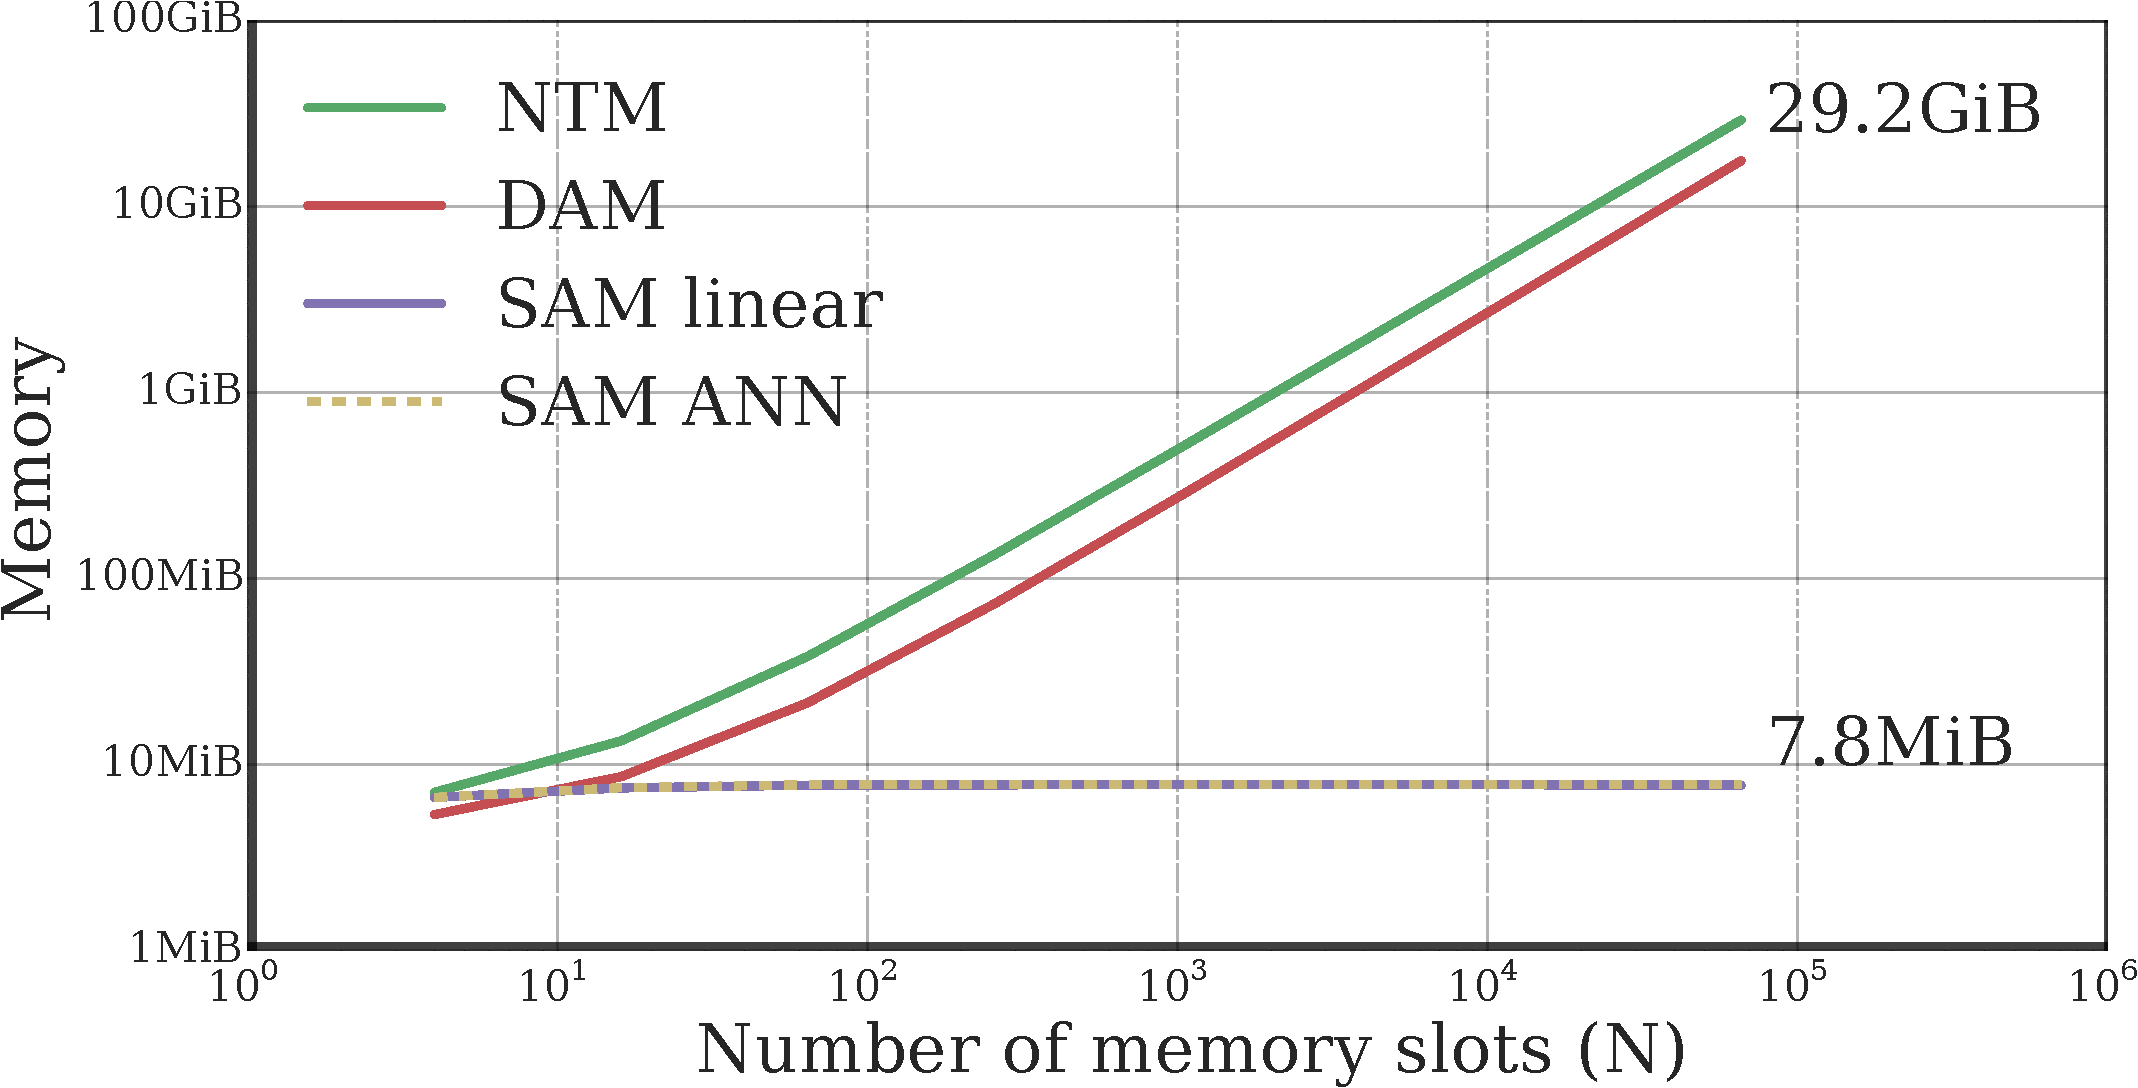
\includegraphics[height=3.4cm]{F_B_memory.pdf}
    \caption{ \label{sf:memory}}
    \end{subfigure}
    %
    \caption{\textbf{(\subref{sf:speed})} Wall-clock time of a single forward and backward pass. The k-d tree is a FLANN randomized ensemble with 4 trees and 32 checks. For 1M memories a single forward and backward pass takes $\SI{12}{s}$ for the NTM and $\SI{7}{ms}$ for SAM, a speedup of $1600\times$.
    \textbf{(\subref{sf:memory})} Memory used to train over sequence of 100 time steps, excluding initialization of external memory. The space overhead of SAM is independent of memory size, which we see by the flat line. When the memory contains 64,000 words the NTM consumes $\SI{29}{GiB}$ whereas SAM consumes only $\SI{7.8}{MiB}$, a compression ratio of $3700$.}
    \label{fig:perf_benchmarks}
\end{figure*}

We measured the forward and backward times of the SAM architecture versus the dense DAM variant and the original NTM (details of setup in Supplementary \ref{sec:benchmarking}). SAM is over $100$ times faster than the NTM when the memory contains one million words and an exact linear-index is used, and $1600$ times faster with the k-d tree (Figure \ref{fig:perf_benchmarks}\subref{sf:speed}). With an ANN the model runs in sublinear time with respect to the memory size. SAM's memory usage per time step is independent of the number of memory words (Figure \ref{fig:perf_benchmarks}\subref{sf:memory}), which empirically verifies the $\mathcal{O}(1)$ space claim from Supplementary \ref{sec:space_time_suppl}. For $\SI{64}{K}$ memory words SAM uses $\SI{53}{MiB}$ of physical memory to initialize the network and $\SI{7.8}{MiB}$ to run a 100 step forward and backward pass, compared with the NTM which consumes $\SI{29}{GiB}$.

%Besides speed, the other constraint that has prevented application of NTM architectures is the memory consumption.

%What this means is that SAM can be trained on much longer sequences than is practical with the NTM.

% TODO (TL): I think it's important to include something like the following caveat:
% Complex memory augmented architectures like the NTM are typically constructed using machine learning libraries such as Torch, Theano, or Tensor Flow because gradients for these models are difficult to compute by hand.
% While convenient, we find that automatic differentiation packages exacerbate the memory usage issue because they often create many internal copies of variables in the computational graph.  So, for example, we found that a straightforward implementation of the NTM architecture in Torch results in more than 10 copies of the external memory being created per time step.  We avoid this issue with SAM by using only inplace operations on the external memory.


%\begin{figure}[H]
%    \centering
%    \includegraphics[width=\columnwidth]{figures/F_B_speed.pdf}
%    \caption{Wall-clock time of a single forward and backward pass. The k-d tree is a FLANN randomized ensemble with 4 trees and 32 checks. For 1M memories a single forward and backward pass takes 12s for the NTM and 7ms for SAM, a speedup of $1600\times$.}
%    \label{fig:speed}
%\end{figure}

% Decided to simplify things and just use the F+B measurements, as they tell the more interesting story.
% Also decided to present this data within a table.
%\begin{figure}[H]
%    \centering
%    \begin{subfigure}[b]{100px}
%        \includegraphics[width=100px]{FB_memory.pdf}
%        \caption{ \label{sf:mem_with_init}}
%    \end{subfigure}
%    \begin{subfigure}[b]{100px}
%        \includegraphics[width=100px]{FB_memory_noinit.pdf}
%        \caption{\label{sf:mem_without_init}}
%    \end{subfigure}
%    \caption{(\subref{sf:mem_with_init}) Memory consumption during training over 100 time steps. This includes network and memory initialization, a forward pass over 100 steps and backpropagation over 100 steps. When the external memory has 64K slots SAM consumes 48MiB vs the NTM's 29Gib, a compression ratio of over 600.  (\subref{sf:mem_without_init}) Memory consumption for only the forward and backward pass, we see the space complexity of SAM per time step is independent of $N$ which explains its overhead. Network architectures are the same as Figure \ref{fig:speed}.}
%    \label{fig:memory}
%\end{figure}

%\begin{table}[H]
%    \centering
%    \begin{tabular}{c | r r c }
%        N       & NTM   & DAM  & SAM  \\
%        \hline
%        256     & 134   & 72    & 7.8 \\
%        1024    & 507   & 274   & 7.8 \\
%        4096    & 1951  & 1087  & 7.8 \\
%        16384   & 7541  & 4335  & 7.8 \\
%        65536   & 29160 & 17329 & 7.8 \\
%    \end{tabular}
%    \caption{Memory used (MB) training over 100 time steps, excluding initialization of external memory. The space overhead of SAM is independent of memory size, leading to a compression ratio of $3700$ relative to the NTM when the memory contains 64K words. }
%    \label{tab:memory}
%\end{table}

%5. Engineering figure -- show memory and speed comparisons versus 'naive' implementations of the dense versions. NTM comparison plot for one task with wall time on x axis - associative recall.


\subsection{Learning with sparse memory access}

\label{ss:ntm_tasks}

We have established that SAM reaps a huge computational and memory advantage of previous models, but can we really learn with SAM's sparse approximations? We investigated the learning cost of inducing sparsity, and the effect of placing an approximate nearest neighbor index within the network, by comparing SAM with its dense variant DAM and some established models, the NTM and the LSTM.

We trained each model on three of the original NTM tasks \cite{graves2014neural}. \textbf{1. Copy}: copy a random input sequence of length 1--20, \textbf{2. Associative Recall}: given 3-6 random (key, value) pairs, and subsequently a cue key, return the associated value. \textbf{3. Priority Sort}: Given 20 random keys and priority values, return the top 16 keys in descending order of priority. We chose these tasks because the NTM is known to perform well on them.

% \textbf{3. Dynamic Ngrams}: Given a sample of 200 bits sampled from an underlying 5-gram distribution, generate samples with low likelihood.

%\begin{itemize}[itemsep=0pt, topsep=0pt, partopsep=0pt]
%\item \textbf{Copy}. Copy a random input sequence of length 1--20.
%\item \textbf{Associative Recall}. Given 3-6 random (key, value) pairs, and subsequently a cue key, return the associated value.
%\item \textbf{Dynamic Ngrams}. Learn to infer the underlying ngram distribution from a sample of 200 bits and make Bayes-optimal predictions.
%\item \textbf{Priority Sort}. Given 20 random keys and priority values, return the top 16 keys in descending order of priority.
%\end{itemize}

Figure \ref{fig:ntm_tasks} shows that sparse models are able to learn with comparable efficiency to the dense models and, surprisingly, learn more effectively for some tasks --- notably priority sort and associative recall. This shows that sparse reads and writes can actually benefit early-stage learning in some cases.

Full hyperparameter details are in Supplementary \ref{sec:training_details}.

%For the dynamic ngram task we do see a reduced final accuracy when using the k-d tree. We think this is because the task's average cost is sensitive to misses during lookup, which the k-d tree is more likely to make. This could be mitigated by investigating ANNs with better accuracy tradeoffs.

\begin{figure*}
    \centering
    % copy
    \begin{subfigure}{0.32\textwidth}
    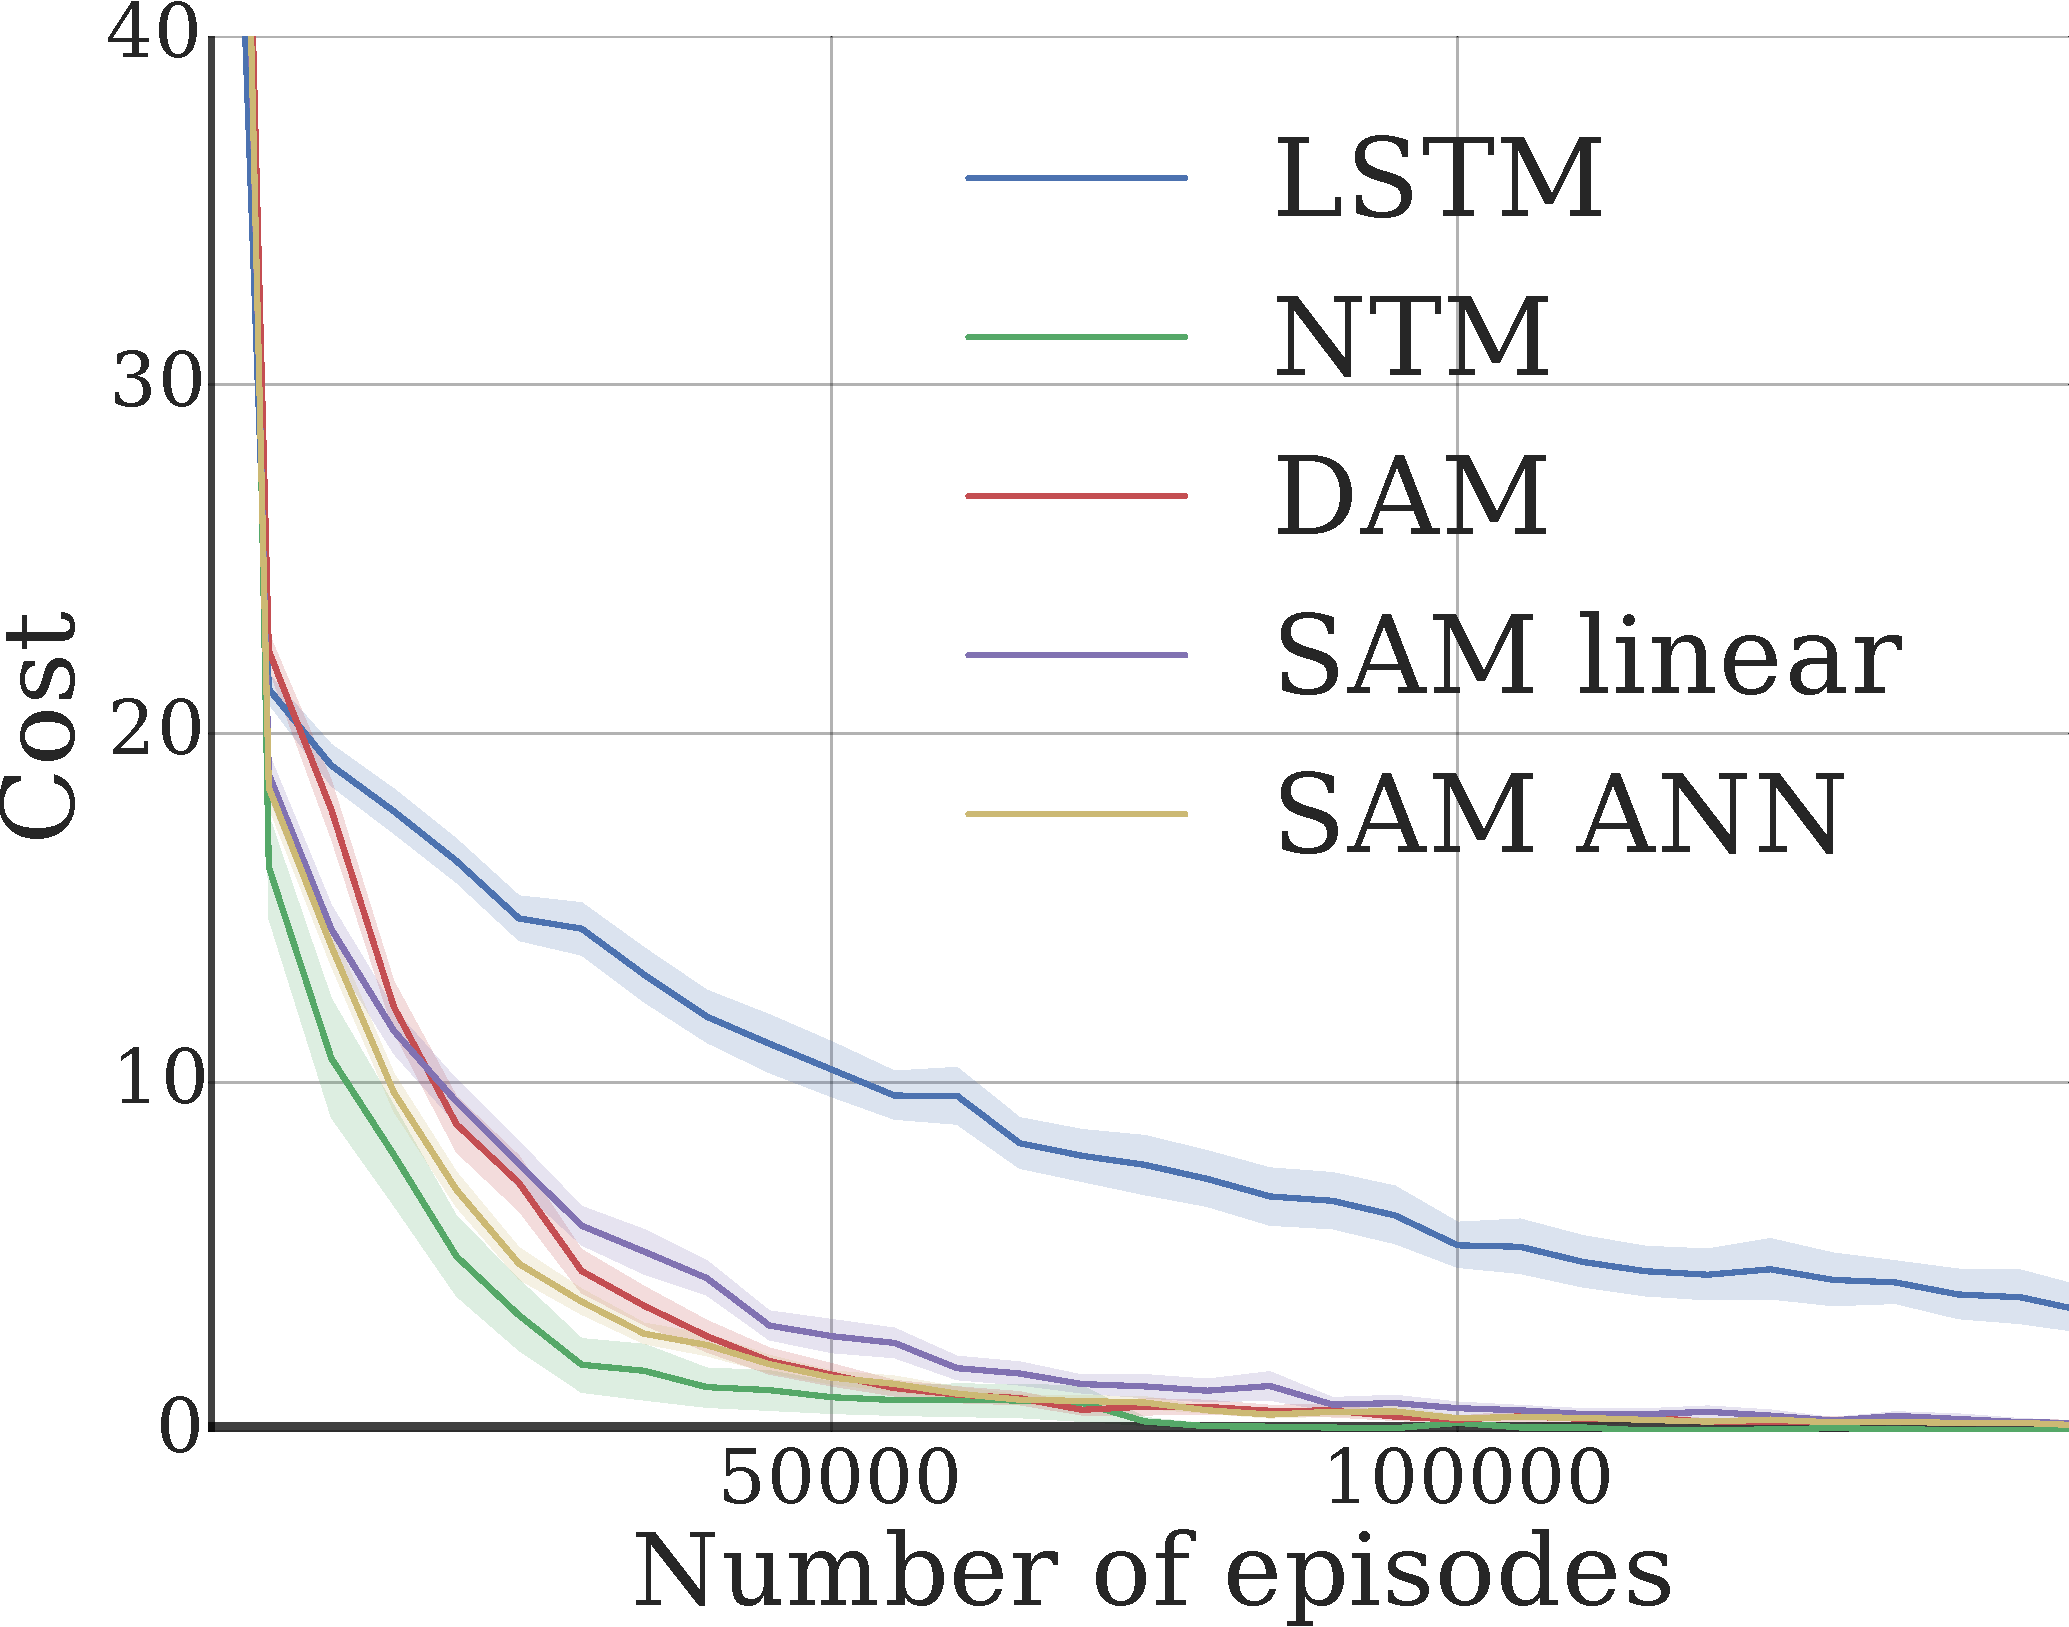
\includegraphics[width=\linewidth]{copy.pdf}
    \caption{ \label{sf:ntm_copy} Copy}
    \end{subfigure}
    %
    % associative recall
    \begin{subfigure}{0.32\textwidth}
    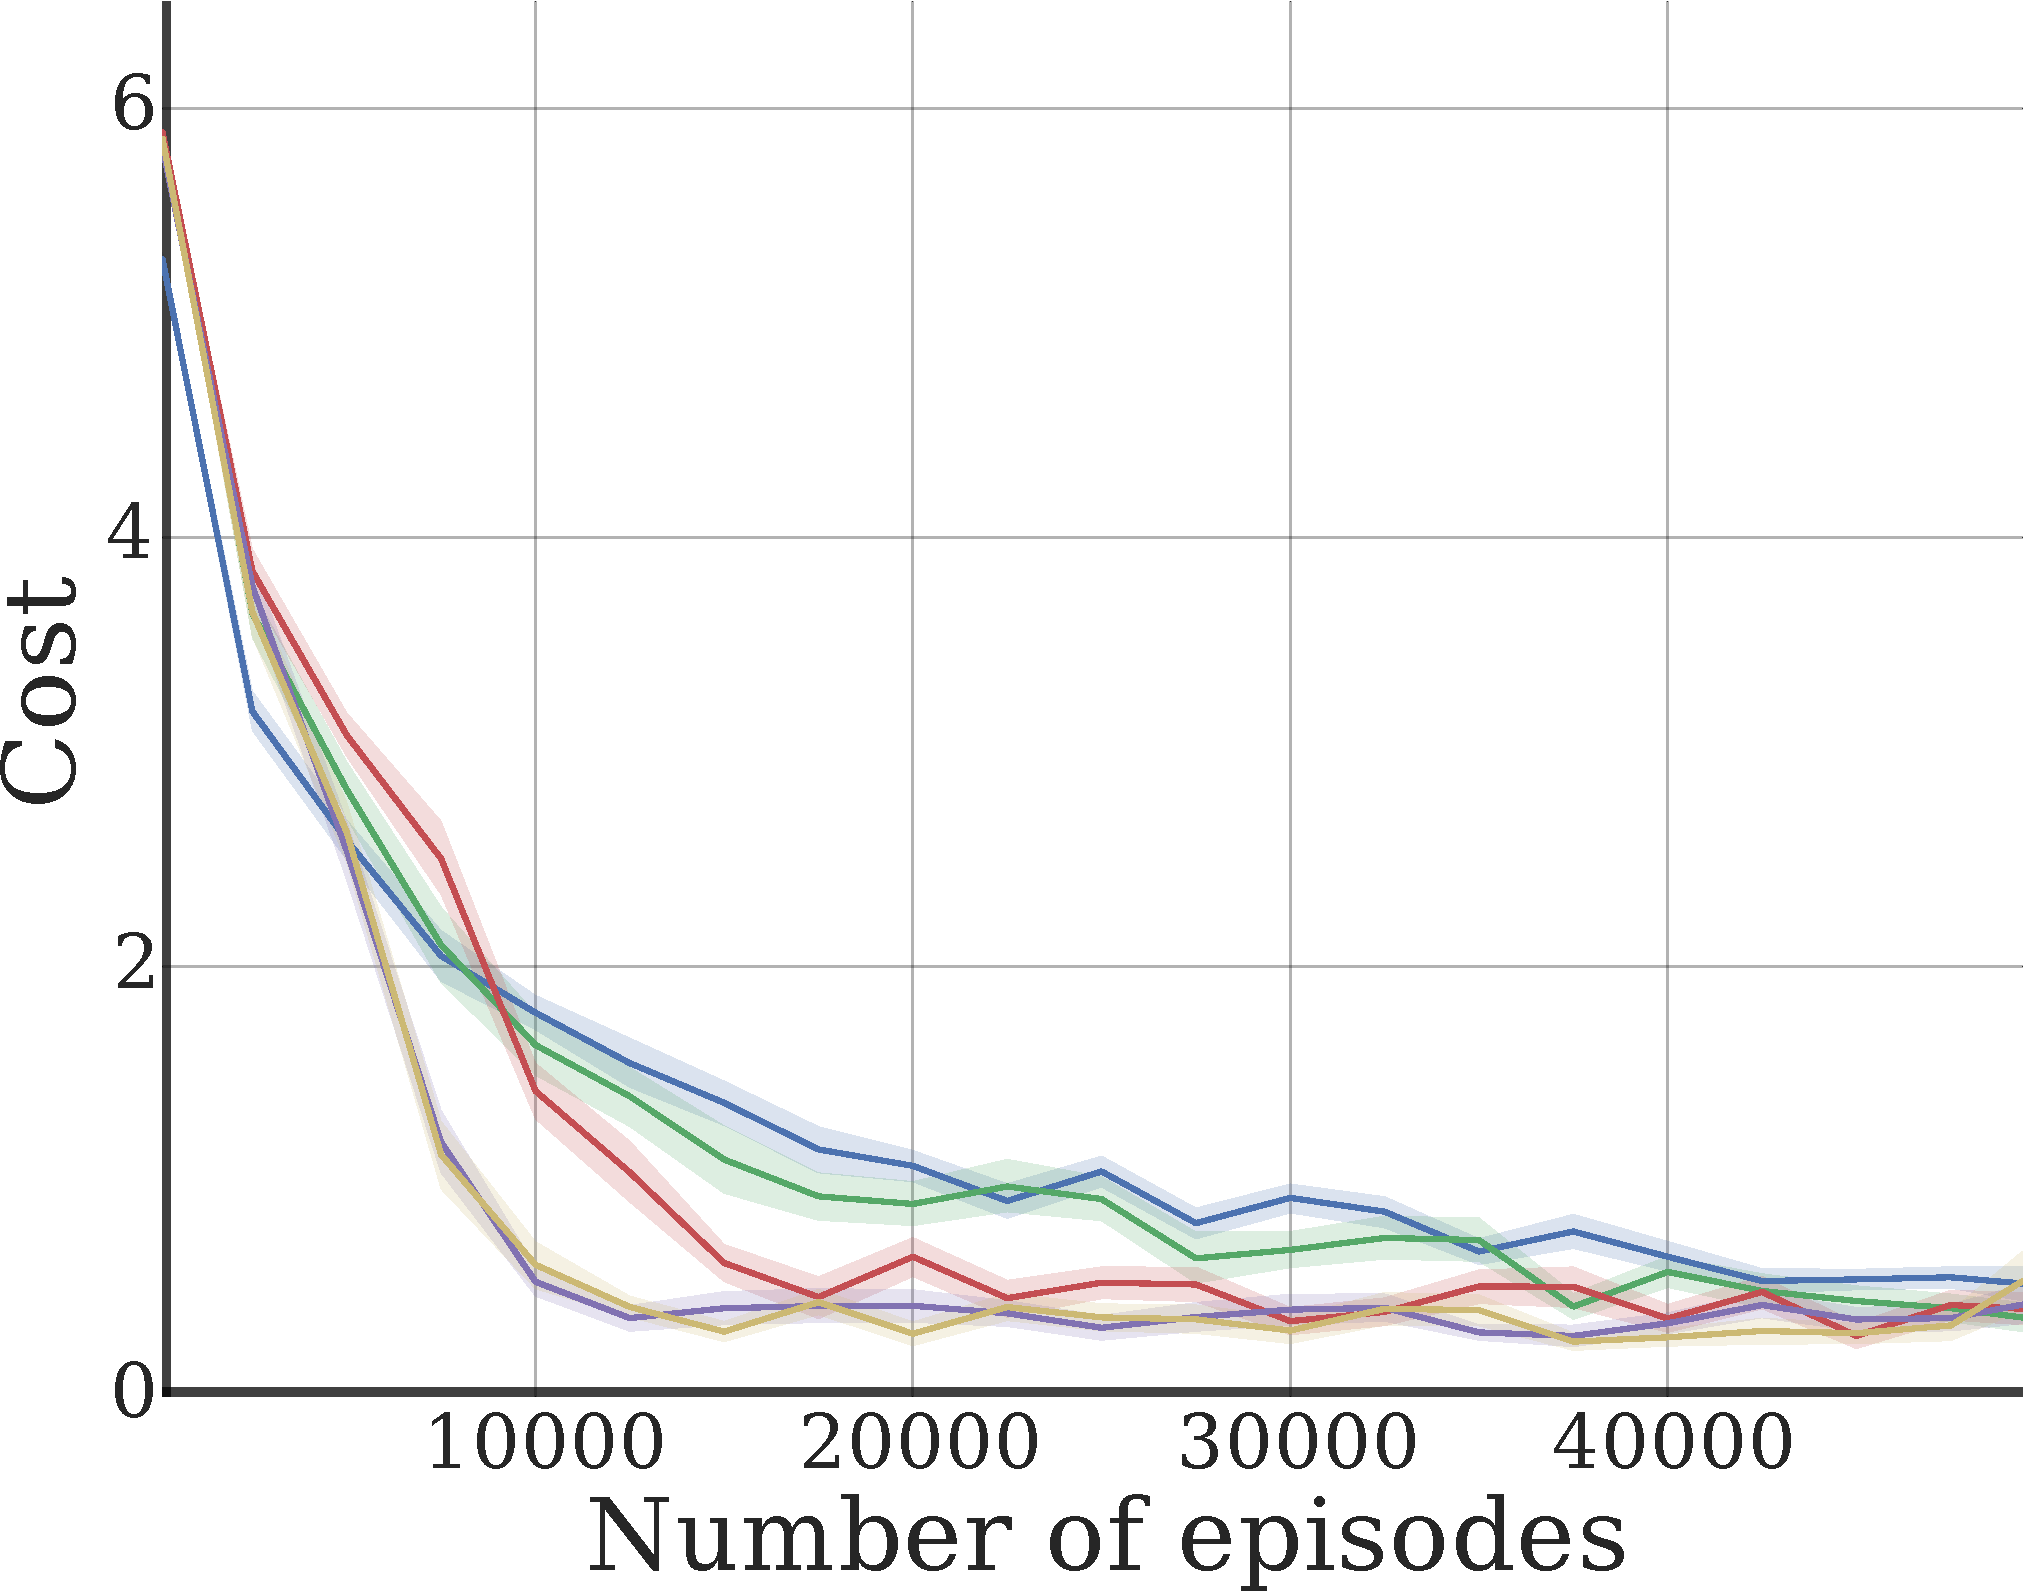
\includegraphics[width=\linewidth]{associativeList.pdf}
    \caption{ \label{sf:ntm_associative_recall} Associative Recall}
    \end{subfigure}
    %
    % dynamic ngrams
    %\begin{subfigure}{0.22\textwidth}
    %\includegraphics[width=\linewidth]{figures/ngram.pdf}
    %\caption{ \label{sf:ntm_ngram}}
    %\end{subfigure}
    %
    % priority sort
    \begin{subfigure}{0.32\textwidth}
    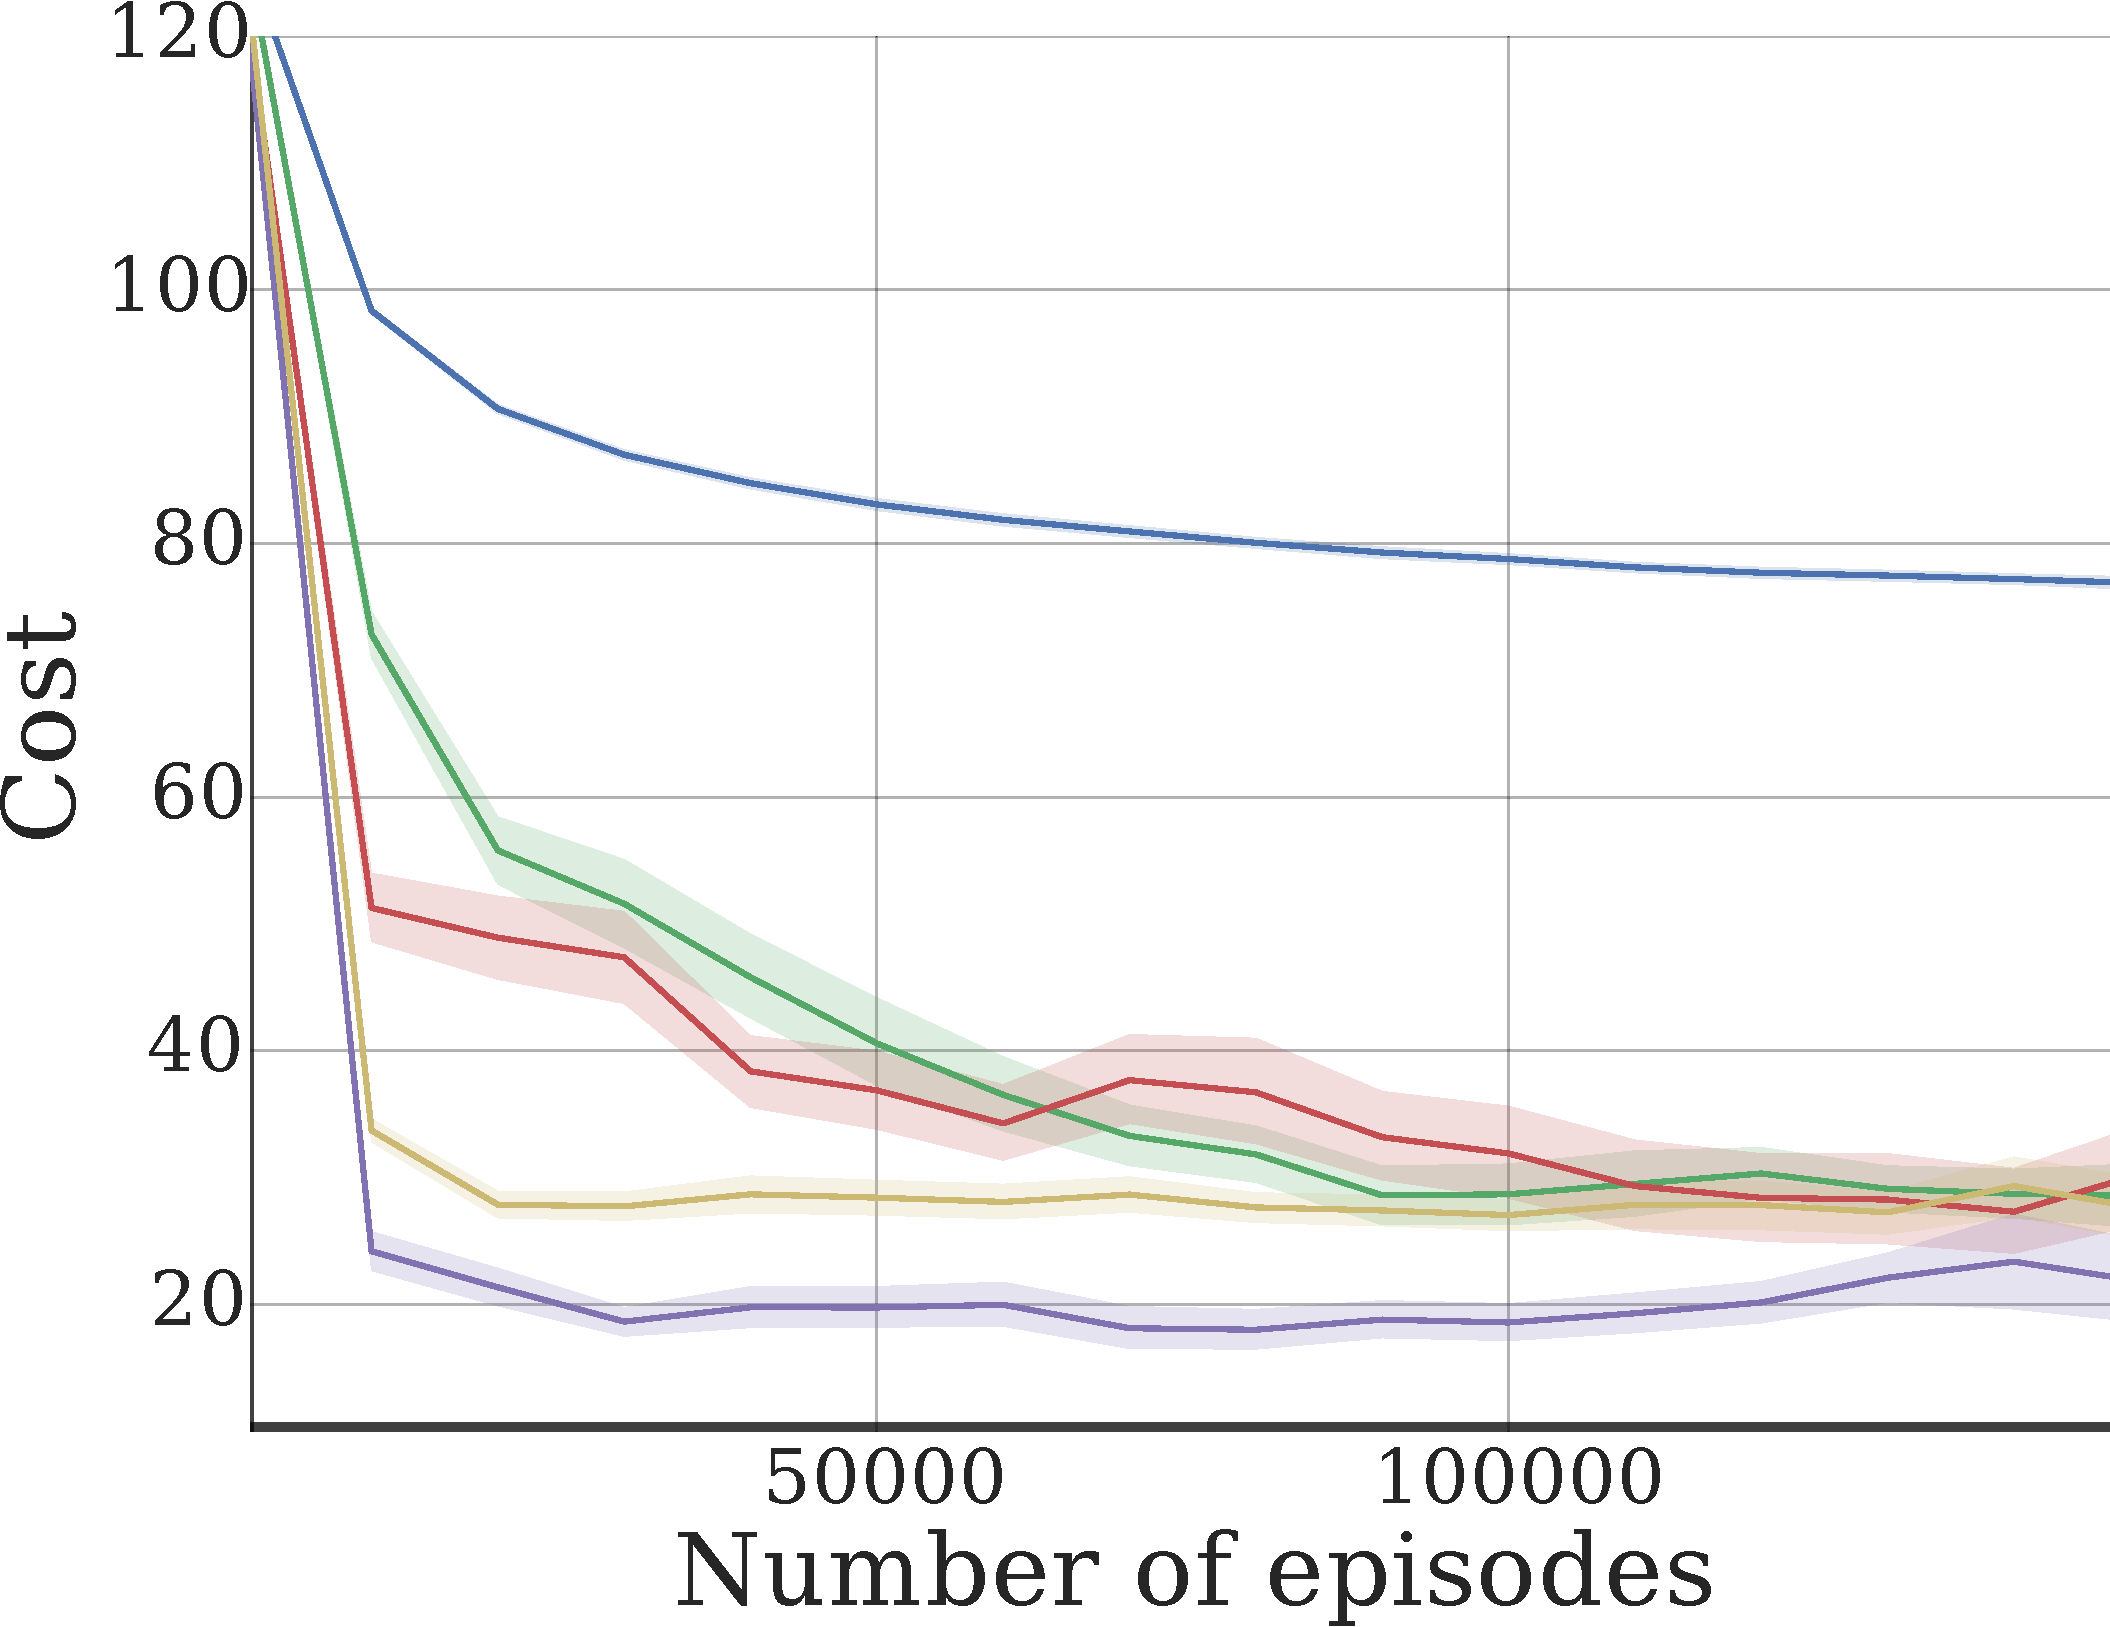
\includegraphics[width=\linewidth]{topk.pdf}
    \caption{ \label{sf:ntm_topk} Priority Sort}
    \end{subfigure}
    %
    \caption{Training curves for sparse (SAM) and dense (DAM, NTM) models. SAM trains comparably for the Copy task, and reaches asymptotic error significantly faster for Associative Recall and Priority Sort.%Panels show the learning curves for three tasks from \cite{graves2014neural}.
    Light colors indicate one standard deviation over 30 random seeds.}
    \label{fig:ntm_tasks}
    % (\subref{sf:ntm_ngram}) dynamic ngrams,
\end{figure*}


\subsection{Scaling with a curriculum}

The computational efficiency of SAM opens up the possibility of training on tasks that require storing a large amount of information over long sequences. Here we show this is possible in practice, by scaling tasks to a large scale via an exponentially increasing curriculum.

%As has been previously noted \cite{bengio2009curriculum,zaremba2014learning,kurach2015neural}, the use of a curriculum is important for training on long sequences.
%Even with our optimizations it is prohibitively slow to train from the beginning on long sequences.
%Additionally, the gradients for long sequences may be noisy.
We parametrized three of the tasks described in Section \ref{ss:ntm_tasks}: associative recall, copy, and priority sort, with a progressively increasing difficulty level which characterises the length of the sequence and number of entries to store in memory. For example, level specifies the input sequence length for the copy task.
We exponentially increased the maximum level $h$ when the network begins to learn the fundamental algorithm.
Since the time taken for a forward and backward pass scales $\mathcal{O}(T)$ with the sequence length $T$, following a standard linearly increasing curriculum could potentially take $\mathcal{O}(T^2)$, if the same amount of training was required at each step of the curriculum.
Specifically, $h$ was doubled whenever the average training loss dropped below a threshold for a number of episodes. The level was sampled for each minibatch from the uniform distribution over integers $\mathcal{U}(0, h)$.

We compared the dense models, NTM and DAM, with both SAM with an exact nearest neighbor index (SAM linear) and with locality sensitive hashing (SAM ANN). The dense models contained 64 memory words, while the sparse models had $2 \times 10^6$ words. These sizes were chosen to ensure all models use approximately the same amount of physical memory when trained over 100 steps.


%The amount of physical memory required for a training episode of length 100 is approximately the same for these memory sizes, so we are comparing roughly equivalent physical memory usage.


%TODO jack & jj, potentially reinclude this paragraph but talk in person first.
%

For all tasks, SAM was able to advance further than the other models, and in the associative recall task, SAM was able to advance through the curriculum to sequences greater than $4000$ (Figure \ref{fig:curriculumT}). Note that we did not use truncated backpropagation, so this involved BPTT for over $4000$ steps with a memory size in the millions of words.

%Note as well that the use of an ANN does not appear to significantly change the data efficiency of learning.
%Using an ANN did appear to improve data efficiency in the associative task, while impairing it slightly in the others, although we found that this was somewhat sensitive to the learning rate.

To investigate whether SAM was able to learn algorithmic solutions to tasks, we investigated its ability to generalize to sequences that far exceeded those observed during training. Namely we trained SAM on the associative recall task up to sequences of length $10,000$, and found it was then able to generalize to sequences of length $200,\!000$ (Supplementary Figure  \ref{fig:extrapolation}). %Despite SAM's memory operations being smooth, we see it remains robust and accurate during sequences of unprecedented length.

%Due to their much smaller memory sizes, the dense models cannot generalize to such long sequences.

%Because training on the curriculum tasks slows downs as the sequence lengths grows, the ANN does not provide a computational speedup during learning on the synthetic task (though this may also be because our ANN implementation has not been well optimized).

%TODO(jjhunt) move to discussion or remove?
%For these benchmarks, we always perform BPTT over the entire sequence. As such, during training the number of memory words used remained below a regime where ANNs provide significant benefits (e.g. $< 16,000$). However, we have seen that the ANN models are able to generalize to much longer sequences. In large-scale practical applications where online learning is used, data can accumulate in the memory over long periods of time. In this scenario, the asymptotic speedups of the ANN (see figure \ref{fig:speed}) will become vital.

%However, we've already seen that the ANN models do generalize to much longer sequences.
%, where the asymptotic speedups of the ANN may become vital.
%since the number of memory words used remains relatively moderate
%(this may also be because our LSH implementation has not been optimized).
%And the setting for the synthetic tasks is quite artificial, in the sense that BPTT is always done over the entire sequence length.



\begin{figure*}[h]
    %\advance\leftskip+3cm
    %\advance\rightskip-3cm
    \begin{minipage}[h]{0.32\textwidth}
        \centering
        % From https://colab.corp.google.com/v2/notebook#fileId=0B3o-wCQ_1oEwNVBsMndkZmVvOHc&scrollTo=Wj0HYm9rNx4k
        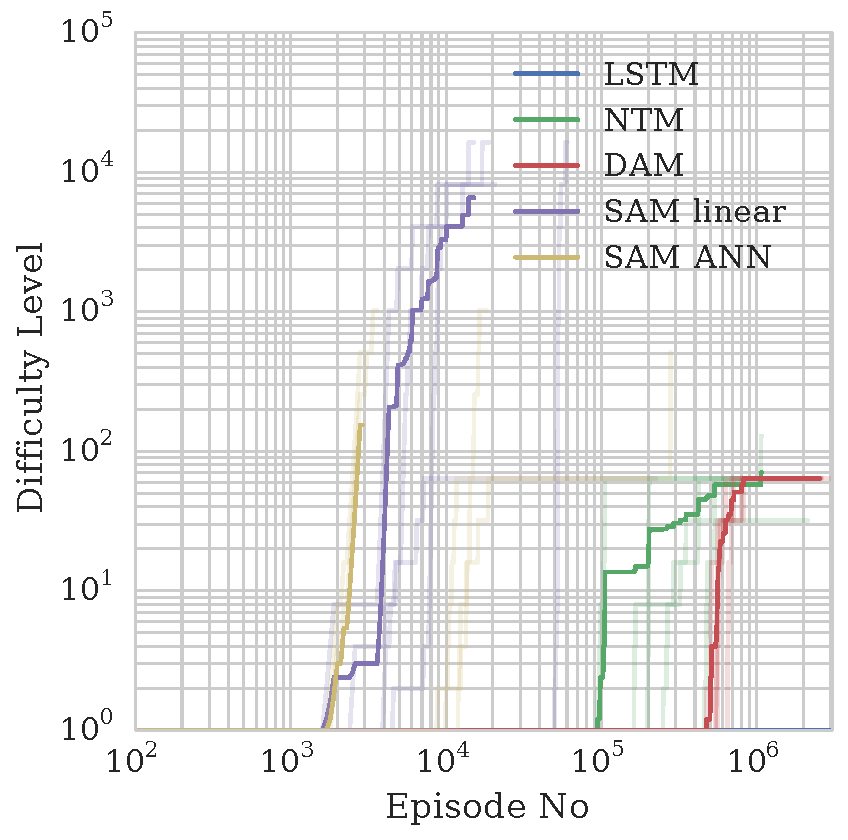
\includegraphics[width=\linewidth]{associativePairsCurriculumlsh3nipsb}
        \subcaption{\label{sf:apc}}
    \end{minipage} %
    %\vspace{-2em}
    \begin{minipage}[h]{0.32\textwidth}
        \centering
        %https://colab.corp.google.com/v2/notebook#fileId=0B3o-wCQ_1oEwTWlpX05salJvR3M&scrollTo=m3f-bU9WNyem
        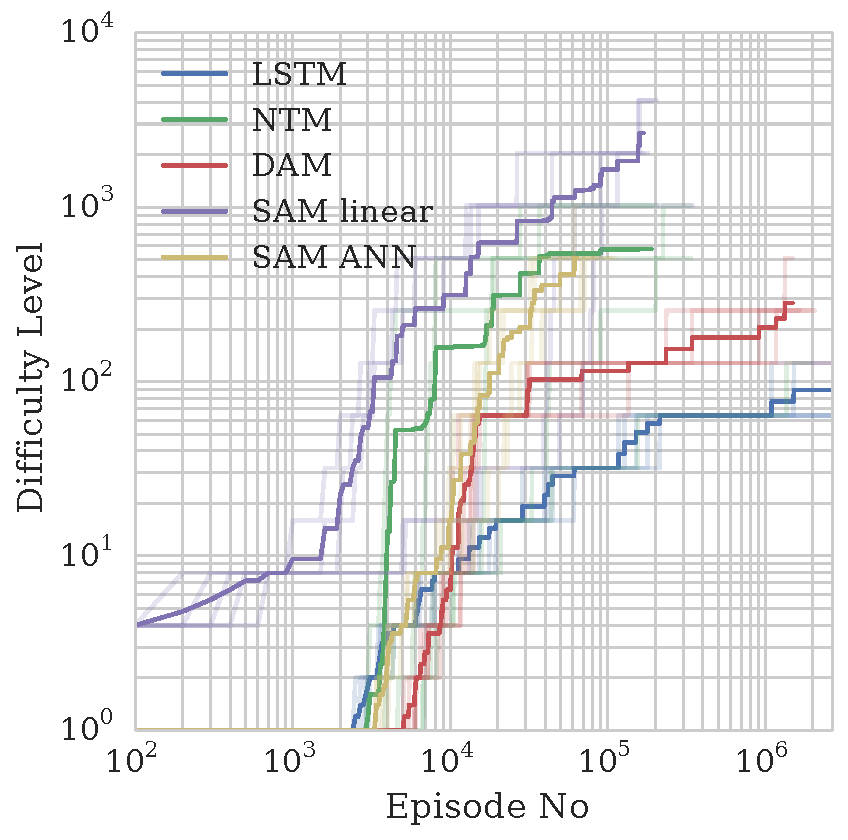
\includegraphics[width=\linewidth]{copyCurriculumlsh3nipsb}
        \subcaption{\label{sf:cc}}
    \end{minipage} %
    %\vspace{-2em}
    \begin{minipage}[h]{0.32\textwidth}
        \centering
        % https://colab.corp.google.com/v2/notebook#fileId=0B3o-wCQ_1oEweGdXMi1MU2JrNTA&scrollTo=TverZ4YWNytF
        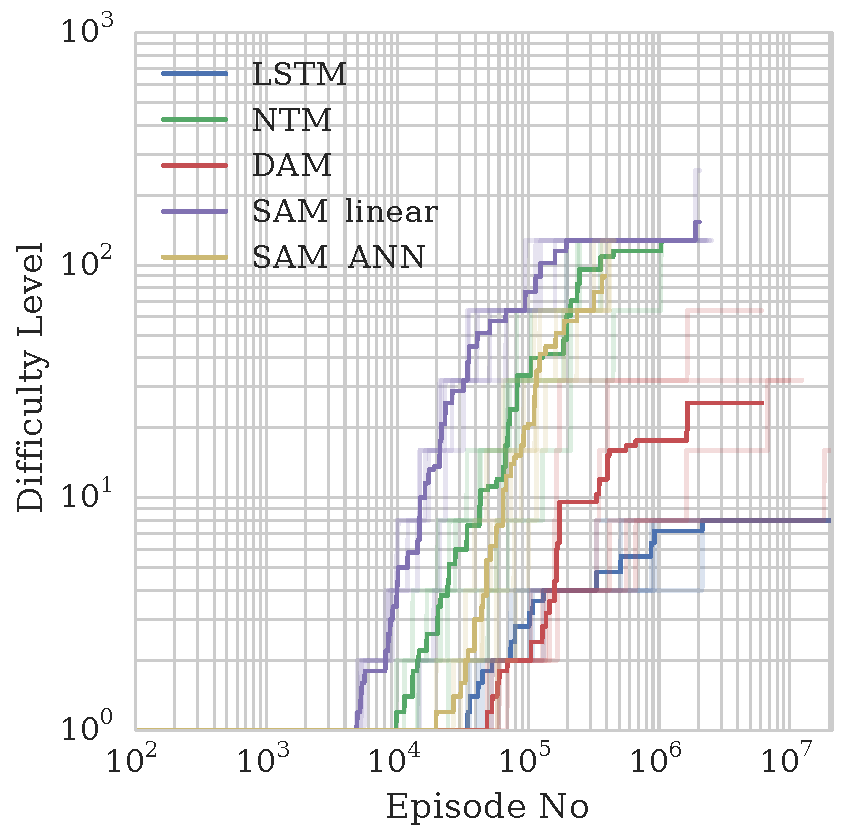
\includegraphics[width=\linewidth]{topkCurriculumlsh3nipsb}
        \subcaption{\label{sf:topkc}}
    \end{minipage}
    \\
    \caption{Curriculum training curves for sparse and dense models on (\subref{sf:apc}) Associative recall, (\subref{sf:cc}) Copy, and (\subref{sf:topkc}) Priority sort. Difficulty level indicates the task difficulty (e.g. the length of sequence for copy). We see SAM train (and backpropagate over) episodes with thousands of steps, and tasks which require thousands of words to be stored to memory. Each model is averaged across 5 replicas of identical hyper-parameters (light lines indicate individual runs).
    }
%    %We trained all of the models on 3 NTM algorithm tasks with curriculum. All of the models received the same amount of computational time and used an exponential curriculum.
%
%    %Note that since we did not perform truncated BPTT, the models run slower as the curriculum advances.
%    %The LSTM runs much faster than other models, but reaches a plateau in performance so, unlike the other models, we do not show the full results for the LSTM.
    \label{fig:curriculumT}
\end{figure*}

\subsection{Question answering on the Babi tasks}

\cite{weston2015towards} introduced toy tasks they considered a prerequisite to agents which can reason and understand natural language. They are synthetically generated language tasks with a vocab of about 150 words that test various aspects of simple reasoning such as deduction, induction and coreferencing.

We tested the models (including the Sparse Differentiable Neural Computer described in Supplementary \ref{sec:sdnc}) on this task. The full results and training details are described in Supplementary \ref{sec:babi}.

The MANNs, except the NTM, are able to learn solutions comparable to the previous best results, failing at only 2 of the tasks. The SDNC manages to solve all but 1 of the tasks, the best reported result on Babi that we are aware of.

Notably the best prior results have been obtained by using supervising the memory retrieval (during training the model is provided annotations which indicate which memories should be used to answer a query). More directly comparable previous work with end-to-end memory networks, which did not use supervision \cite{sukhbaatar2015end}, fails at 6 of the tasks.

Both the sparse and dense perform comparably at this task, again indicating the sparse approximations do not impair learning. We believe the NTM may perform poorly since it lacks a mechanism which allows it to allocate memory effectively.


%\begin{table}[]
%    \centering
%    \begin{tabular}{l|c|c|c|c|c|c|c|c|c}
% Table autogenerated from run 53.
% https://colab.corp.google.com/v2/notebook#fileId=0B3o-wCQ_1oEwOEZ1S0tuM25uanM&scrollTo=U93IbZ_ryJpQ
%  & LSTM & SparseMeta & SAM & DAM & NTM & DenseMeta & Best Previous & Human \\
%\hline
%Named entities  & $0.374$ & $0.394$ & $0.403$ & $0.403$ & $0.376$ & $0.393$ & $0.666$ & $0.816 \\
%Common Nouns  & $0.326$ & $0.365$ & $0.370$ & $0.358$ & $0.313$ & $0.333$ & $0.630$ & $0.816 \\
%Verbs  & $0.592$ & $0.611$ & $0.631$ & $0.620$ & $0.553$ & $0.579$ & $0.818$ & $0.828 \\
%Prepositions  & $0.683$ & $0.692$ & $0.698$ & $0.680$ & $0.643$ & $0.676$ & $0.806$ & $0.708 \\
% End of autogenerated
%    \end{tabular}
%    \caption{CBT best results}
%    \label{tab:babi_best}
%\end{table}

\subsection{Learning on real world data}

Finally, we demonstrate that the model is capable of learning in a non-synthetic dataset. Omniglot \cite{lake2015human} is a dataset of 1623 characters taken from 50 different alphabets,
with 20 examples of each character.
This dataset is used to test rapid, or \textit{one-shot} learning, since there are few examples of each character but many different character classes. Following \cite{santoro2016}, we generate episodes where a subset of characters are randomly selected from the dataset, rotated and stretched, and assigned a randomly chosen label. At each time step an example of one of the characters is presented, along with the correct label of the proceeding character. Each character is presented 10 times in an episode (but each presentation may be any one of the 20 examples of the character). In order to succeed at the task the model must learn to rapidly associate a novel character with the correct label, such that it can correctly classify subsequent examples of the same character class.

Again, we used an exponential curriculum, doubling the number of additional characters provided to the model whenever the cost was reduced under a threshold. After training all MANNs for the same length of time, a validation task with $500$ characters was used to select the best run, and this was then tested on a test set, containing all novel characters for different sequence lengths (Figure \ref{fig:omniglot}). All of the MANNs were able to perform much better than chance, even on sequences $\approx 4\times$ longer than seen during training. SAM outperformed other models, presumably due to its much larger memory capacity. Previous results on the Omniglot curriculum \cite{santoro2016} task are not identical, since we used 1-hot labels throughout and the training curriculum scaled to longer sequences, but our results with the dense models are comparable ($\approx 0.4$ errors with $100$ characters), while the SAM is significantly better ($0.2 <$ errors with $100$ characters).

%We see in Figure \ref{fig:omniglot} that SAM is capable of learning this task with comparable data efficiency to the dense models.

\begin{figure}[h]
  % from https://colab.corp.google.com/v2/notebook#fileId=0B3o-wCQ_1oEwSXNhVlNZTVhkYUk&scrollTo=S3pkcd-Zezm7
  %\includegraphics[width=6cm]{omniglot1ff2b}
  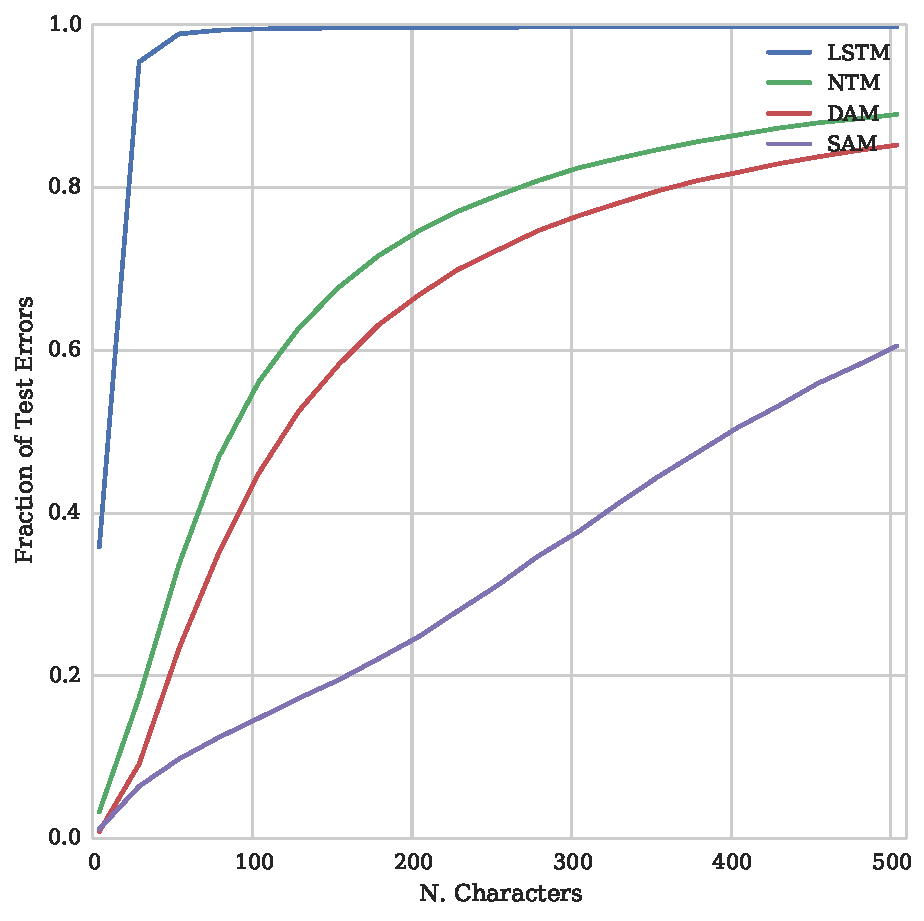
\includegraphics[width=6cm]{omniglot_curriculum_test_extrapolation}
  \caption{Test errors for the Omniglot task (described in the text) for the best runs (as chosen by the validation set). The characters used in the test set were not used in validation or training. All of the MANNs were able to perform much better than chance with $\approx 500$ characters (sequence lengths of $\approx 5000$), even though they were trained, at most, on sequences of $\approx 130$ (chance is $0.002$ for $500$ characters). This indicates they are learning generalizable solutions to the task. SAM is able to outperform other approaches, presumably because it can utilize a much larger memory. }
 % \caption{Curriculum level (number of characters) for the Omniglot one-shot character recognition class. Again, on a task with real data, the sparse approximations do not impair learning. Both DAM and SAM are able to scale to sequences with $\approx 2500$ timesteps. }
  \label{fig:omniglot}
\end{figure}



%\subsection{Related approaches}
%\subsubsection{MemNets}

%\textit{Survey the space and time complexity for several models: NTM, MemNets, LSTM, GRU, Neural GPU.}
%
%\cite{sukhbaatar2015end} TODO memnets
%\cite{kurach2015neural} neural ram
%\cite{bahdanau2014neural} machine translation with alignment (this is very similar to memnets except encoding is sequential, not exactly sure who came first)
%\cite{hill2015goldilocks} TODO goldilocks NLP task
%
%\begin{enumerate}
%\item Introduce the MemNet read operation.
%\item Attention over data (not attention over memories).
%\end{enumerate}
%
%
%
%\subsection{Online memory}
%
%Offline vs online memory, with relevance to KNN stability.
%
%Discussion of RL-based discrete decisions.

%jjhunt proposed intro
% agreed: JJ's is simpler and thus more appropriate here.
% some of the bits above could be moved to the related work section?
% Why focus on content-based systems!?

%The NTM incorporates a combination of content-based and location-based addressing mechanisms.  Architectures such as Neural Stacks are purely location-based. And MemNets are purely content-based.

%We focused on the NTM architecture as it is most similar to SAM, however it's worth noting that the principles of sparse access memory can be equally applied to creating scalable MemNets.

%TODO, need a bit more summing up or something before the memnets discussion, maybe merge the discussion and conclusion into one section.

\section{Discussion}

Scaling memory systems is a pressing research direction due to potential for compelling applications with large amounts of memory. We have demonstrated that you can train neural networks with large memories via a sparse read and write scheme that makes use of efficient data structures within the network, and obtain significant speedups during training. Although we have focused on a specific MANN (SAM), which is closely related to the NTM, the approach taken here is general and can be applied to many differentiable memory architectures, such as Memory Networks \cite{weston2014memory}.

%Memory Networks do not require any mechanism for memory allocation since everything the mechanism for writing the memory is fixed, however the principle of using approximate k-nearest neighbor searching over memory, sparse matrix routines to take advantage of the induced sparsity, and $\mathcal{O}(1)$ backpropagation are equally relevant.

It should be noted that there are multiple possible routes toward scalable memory architectures. For example, prior work aimed at scaling Neural Turing Machines \cite{zaremba2015reinforcement} used reinforcement learning to train a discrete addressing policy. This approach also touches only a sparse set of memories at each time step, but relies on higher variance estimates of the gradient during optimization. Though we can only guess at what class of memory models will become staple in machine learning systems of the future, we argue in Supplementary \ref{sec:space_time_suppl} that they will be no more efficient than SAM in space and time complexity if they address memories based on content.

%We have proved that our model is asymptotically efficient for online, sequential tasks with large memories. Additionally, we have demonstrated empirically that the model is able to learn with similar  data efficiency to dense models on 4 synthetic tasks. We also demonstrated that it is able to extrapolate and solve sequential tasks with 100,000s of time steps, which is substantially longer than previously demonstrated.

%\cite{martins2016softmax}


%In the NTM, the location-based addressing mechanism serves as a way of allocating new memory to write to.  Since we have only content-based access, but still read and write to memory over multiple time steps, we introduce a mechanism that allows the controller to allocate new memory.  Memory is allocated by tracking how often a memory slot has been accessed and then providing a mechanism for the controller to write to the least recently accessed memory for writing.

We have experimented with randomized k-d trees and LSH within the network to reduce the forward pass of training to sublinear time, but there may be room for improvement here. K-d trees were not designed specifically for fully online scenarios, and can become imbalanced during training. Recent work in tree ensemble models, such as Mondrian forests \cite{lakshminarayanan2014mondrian}, show promising results in maintaining balanced hierarchical set coverage in the online setting. An alternative approach which may be well-suited is LSH forests \cite{bawa2005lsh}, which adaptively modifies the number of hashes used. It would be an interesting empirical investigation to more fully assess different ANN approaches in the challenging context of training a neural network.

Humans are able to retain a large, task-dependent set of memories obtained in one pass with a surprising amount of fidelity \cite{brady2008visual}. Here we have demonstrated architectures that may one day compete with humans at these kinds of tasks.
%begin to show promise of competing with humans at this. %, and enable recurrent architectures which require large amounts of context.


% TODO talk more about other approaches etc.

%Here we examine a particular sparse memory architecture in which both the read and write operations are content-based. In this sense the architecture is similar to MemNets, but unlike MemNets and similar to NTMs we do allow a recurrent controller to access memory for reading and writing at every time step.  By incorporating a recurrent controller that accesses memory sequentially, the architecture is able to perform tasks that are irredeemably sequential, such as in the case of interacting with an environment in a reinforcement learning task.


%Humans and animals have large capacity one-shot memory stores that are content addressable and that they use to facilitate many behaviours.
%Recently introduced models, neural turning machines and memory networks, have suggested architectures that give neural networks access to external memory stores that can be searched by content.  In the case of the neural turning machine, a recurrent controller writes to and reads from a memory store using operations which are fully differentiable.  This makes the models tractable for end-to-end gradient based learning.
%Unfortunately, these models cannot make use of very large capacity memories due to the fact that content based search scales linearly with the size of the memory.



%\subsection{Conclusion}

% TODO cite some more human. shorten


\subsection*{Acknowledgements}
We thank Vyacheslav Egorov, Edward Grefenstette, Malcolm Reynolds, Fumin Wang and Yori Zwols for their assistance, and the Google DeepMind family for helpful discussions and encouragement.

\small
\bibliography{example_paper}{}
\bibliographystyle{plain}

\newpage
\appendix

\section*{Supplementary Information}

\section{Time and space complexity}
\label{sec:space_time_suppl}

Under a reasonable class of content addressable memory architectures $\mathcal{A}$, SAM is optimal in time and space complexity.

\begin{definition}
\label{label:def_cam}
Let $\mathcal{M}$ be a collection of real vectors $m_1, m_2, \ldots, m_N$ of fixed dimension $d$. Let $\mathcal{A}$ be the set of all content addressable memory data structures that store $\mathcal{M}$ and can return at least one word $m_j$ such that $D(q, m_j) \le c \, (1 + \epsilon) $ for a given $L^p$ norm $D$, query vector $q$, and $\epsilon > 0$; provided such a memory $m_c \,$ exists with $D(q, m_c) = c$.
\end{definition}

Existing lower bounds \cite{motwani2007lower,arya1998optimal} assert that for any data structure $a \in \mathcal{A}$, $a$  requires $\Omega(\log N)$ time and $\Omega(N)$ space to perform a read operation. The SAM memory architecture proposed in this paper is contained within $\mathcal{A}$ as it computes the approximate nearest neighbors problem in fixed dimensions \cite{flann_pami_2014}. As we will show, SAM requires $\mathcal{O}(\log N)$ time to query and maintain the ANN, $\mathcal{O}(1)$ to perform all subsequent sparse read, write, and error gradient calculations. It requires $\mathcal{O}(N)$ space to initialize the memory and $\mathcal{O}(1)$ to store intermediate sparse tensors. We thus conclude it is optimal in asymptotic time and space complexity.


\subsection{Initialization}
Upon initialization, SAM consumes $\mathcal{O}(N)$ space and time to instantiate the memory and the memory Jacobian. Furthermore, it requires $\mathcal{O}(N)$ time and space to initialize auxiliary data structures which index the memory, such as the approximate nearest neighbor which provides a content-structured view of the memory, and the least accessed ring, which maintains the temporal ordering in which memory words are accessed. These initializations represent an unavoidable one-off cost that does not recur per step of training, and ultimately has little effect on training speed. For the remainder of the analysis we will concentrate on the space and time cost per training step.
\subsection{Read}
Recall the sparse read operation,

\begin{equation}
\label{eq:sparse_read_suppl}
\tilde r_t = \sum_{i = 1}^K   \tilde w_t^R(s_i) \mathbf{M}_t (s_i) \; .
\end{equation}

As $K$ is chosen to be a fixed constant, it is clear we can compute (\ref{eq:sparse_read_suppl}) in $\mathcal{O}(1)$ time. During the backward pass, we see the gradients are sparse with only $K$ non-zero terms,
\[
\frac{\partial L}{\partial \tilde  w^R_t}(i) =
\left \{
    \begin{array}{ll}
        \mathbf{M}_t(i) \cdot \frac{\partial L}{\partial \tilde r_t} & \hbox{if } i \in \{s_1, s_2, \ldots, s_K\} \\
        0 & \hbox{otherwise.}
    \end{array}
\right .
\]
and
\[
\frac{\partial L}{\partial  M_t}(i) =
\left \{
    \begin{array}{ll}
        \tilde w^R_t(i) \frac{\partial L}{\partial \tilde r_t} & \hbox{if } i \in \{s_1, s_2, \ldots, s_K\} \\
        \mathbf{0} & \hbox{otherwise.}
    \end{array}
\right .
\]
where $\mathbf{0}$ is a vector of $M$ zeros. Thus they can both be computed in constant time by skipping the computation of zeros. Furthermore by using an efficient sparse matrix format to store these matrices and vectors, such as the CSR, we can represent them using at most $3K$ values. Since the read word $\tilde r_t$ and its respective error gradient is the size of a single word in memory ($M$ elements), the overall space complexity is $\mathcal{O}(1)$ per time step for the read.

\subsection{Write}
Recall the write operation,

\begin{equation}
    \label{eq:sparse_write_suppl}
    \mathbf{M}_t \leftarrow \mathbf{M}_{t - 1} - \mathbf{E}_t  + \mathbf{A}_t, \; ,
\end{equation}

where $\mathbf{A}_t = w^{\W}_t a_t^T$ is the add matrix, $\mathbf{E_t} = \mathbf{M}_{t - 1} \odot \mathbf{R}_t$ is the erase matrix, and $\mathbf{R}_t = \mathbb{I}^U_t \mathbf{1}^T$ is defined to be the erase weight matrix. We chose the write weights to be an interpolation between the least recently accessed location and the previously read locations,

\begin{equation}
    \label{eq:lru_write_weights_suppl}
    w^{\W}_t = \alpha_t \, \left( \gamma_t \, \tilde w^R_{t-1} + (1 - \gamma_t) \, \mathbb{I}^U_t \right) \, .
\end{equation}

For sparse reads where $w^{R}_t = \tilde w^{R}_t$ is a sparse vector with $K$ non-zeros, the write weights $w^{\W}_t$ is also sparse with $K + 1$ non-zeros: $1$ for the least recently accessed location and $K$ for the previously read locations. Thus the sparse-dense outer product $\mathbf{A_t} = w^{\W}_t a_t^T$ can be performed in $\mathcal{O}(1)$ time as $K$ is a fixed constant.

Since $\mathbf{R}_t = \mathbb{I}^U_t \mathbf{1}^T$ can be represented as a sparse matrix with one single non-zero, the erase matrix $\mathbf{E}_t$ can also. As $\mathbf{A_t}$ and $\mathbf{E_t}$ are sparse matrices we can then add them component-wise to the dense $\mathbf{M_{t-1}}$ in $\mathcal{O}(1)$ time. By analogous arguments the backward pass can be computed in $\mathcal{O}(1)$ time and each sparse matrix can be represented in $\mathcal{O}(1)$ space.

We avoid caching the modified memory, and thus duplicating it, by applying the write directly to the memory. To restore its prior state during the backward pass, which is crucial to gradient calculations at earlier time steps, we roll the memory it back by reverting the sparse modifications with an additional $\mathcal{O}(1)$ time overhead (Supplementary Figure \ref{fig:bptt}).

The location of the least recently accessed memory can be maintained in $\mathcal{O}(1)$ time by constructing a circular linked list that tracks the indices of words in memory, and preserves a strict ordering of relative temporal access. The first element in the ring is the least recently accessed word in memory, and the last element in the ring is the most recently modified. We keep a ``head'' pointer to the first element in the ring. When a memory word is randomly accessed, we can push its respective index to the back of the ring in $\mathcal{O}(1)$ time by redirecting a small number of pointers. When we wish to pop the least recently accessed memory (and write to it) we move the head to the next element in the ring in $\mathcal{O}(1)$ time.


\begin{figure}[H]
    \centering
    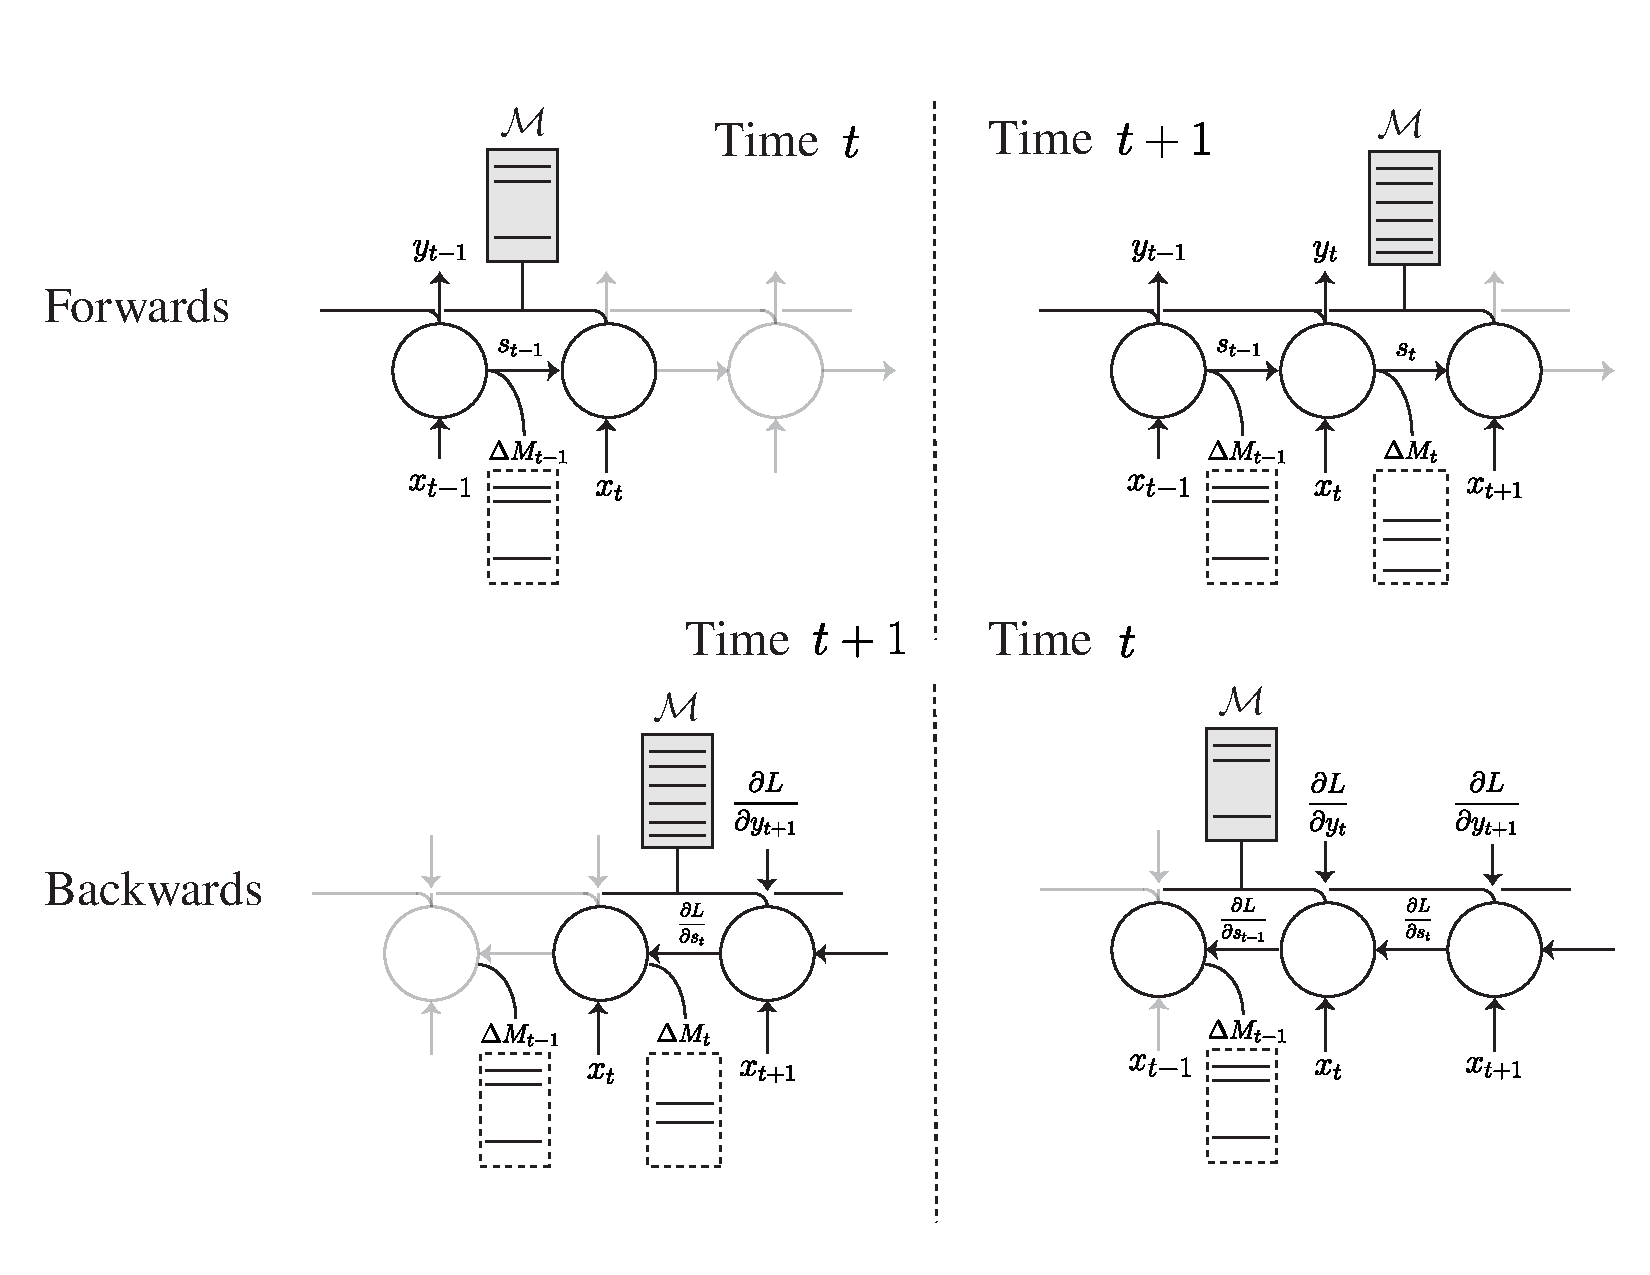
\includegraphics[width=\columnwidth]{Efficient_BPTT.pdf}
    \caption{A schematic of the memory efficient backpropagation through time. Each circle represents an instance of the SAM core at a given time step. The grey box marks the dense memory. Each core holds a reference to the single instance of the memory, and this is represented by the solid connecting line above each core. We see during the forward pass, the memory's contents are modified sparsely, represented by the solid horizontal lines. Instead of caching the changing memory state, we store only the sparse modifications --- represented by the dashed white boxes. During the backward pass, we ``revert'' the cached modifications to restore the memory to its prior state, which is crucial for correct gradient calculations.}
    \label{fig:bptt}
\end{figure}

\subsection{Content-based addressing}
As discussed in Section \ref{sec:ann} we can calculate the content-based attention, or read weights $w^{R}_t$, in $\mathcal{O}(\log N)$ time using an approximate nearest neighbor index that views the memory. We keep the ANN index synchronized with the memory by passing it through the network as a non-differentiable member of the network's state (so we do not pass gradients for it), and we update the index upon each write or erase to memory in $\mathcal{O}(\log N)$ time. Maintaining and querying the ANN index represents the most expensive part of the network, which is reasonable as content-based addressing is inherently expensive \cite{motwani2007lower,arya1998optimal}.

For the backward pass computation, specifically calculating $\frac{\partial L}{\partial q_t}$ and $\frac{\partial L}{\partial \mathbf{M_t}}$ with respect to $w^R_t$, we can once again compute these using sparse matrix operations in $\mathcal{O}(1)$ time. This is because the $K$ non-zero locations have been determined during the forward pass.

Thus to conclude, SAM consumes in total $\mathcal{O}(1)$ space for both the forward and backward step during training, $\mathcal{O}(\log N)$ time per forward step, and $\mathcal{O}(1)$ per backward step.

\section{Control flow}

\begin{figure}[H]
    \centering
    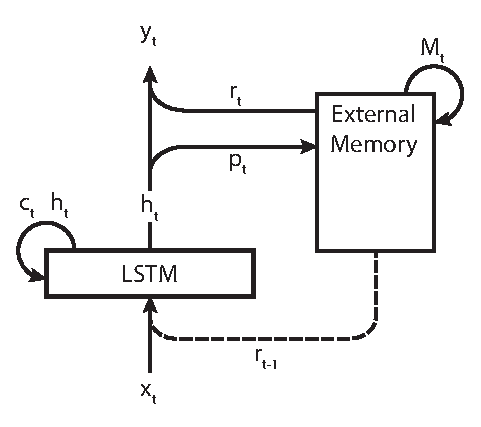
\includegraphics[scale=0.7]{controlflow.eps}
    \caption{Schematic showing how the controller interfaces with the external memory in our experiments. The controller (LSTM) output $h_t$ is used (through a linear projection, $p_t$) to read and write to the memory. The result of the read operation $r_t$ is combined with $h_t$ to produce output $y_t$, as well as being feed into the controller at the next timestep ($r_{t-1}$).}
    \label{fig:controlflow}
\end{figure}

\section{Training details}
\label{sec:training_details}
Here we provide additional details on the training regime used for our experiments used in Figure \ref{fig:ntm_tasks}.

To avoid bias in our results, we chose the learning rate that worked best for DAM (and not SAM). We tried learning rates $\{10^{-6}, 5 \times 10^{-5}, 10^{-5}, 5 \times 10^{-4}, 10^{-4}\}$ and found that DAM trained best with $10^{-5}$. We also tried values of $K$ $\{4, 8, 16\}$ and found no significant difference in performance across the values.  We used 100 hidden units for the LSTM (including the controller LSTMs), a minibatch of $8$, $8$ asynchronous workers to speed up training, and \texttt{RMSProp} \cite{tieleman2012lecture} to optimize the controller. We used $4$ memory access heads and configured SAM to read from only $K = 4$ locations per head.


\section{Sparse Differentiable Neural Computer}
\label{sec:sdnc}

Recently \cite{graves2016dnc} proposed a novel MANN the Differentiable Neural Computer (DNC). The two innovations proposed by this model are a new approach to tracking memory freeness (dynamic memory allocation) and a mechanism for associating memories together (temporal memory linkage).
We demonstrate here that the approaches enumerated in the paper can be adapted to new models by outlining a sparse version of this model, the Sparse Differentiable Neural Computer (SDNC), which learns with similar data efficiency while retaining the computational advantages of sparsity.

\subsection{Architecture}
For brevity, we will only explain the sparse implementations of these two items, for the full model details refer to the original paper. The mechanism for sparse memory reads and writes was implemented identically to SAM.

It is possible to implement a scalable version of the dynamic memory allocation system of the DNC avoiding any $O(N)$ operations by using a heap. However, because it is practical to run the SDNC with many more memory words, reusing memory is less crucial so we did not implement this and used the same usage tracking as in SAM.

The temporal memory linkage in the DNC is a system for associating and recalling memory locations which were written in a temporal order, for exampling storing and retrieving a list. In the DNC this is done by maintaining a temporal linkage matrix $\mathbf{L}_t \in [0, 1]^{N \times N}$. $\mathbf{L}_t[i,j]$ represents the degree to which location $i$ was written to after location $j$. This matrix is updated by tracking the precedence weighting $p_t$, where $p_t(i)$ represents the degree to which location $i$ was written to.
\begin{align}
    p_0 &= 0    \\
    p_t &= (1 - \sum_i w_t^{W}(i) ) \, p_{t-1} + w_t^{W}
\end{align}
The memory linkage is updated according to the following recurrence
\begin{align}
\mathbf{L}_0 &= 0 \\
\mathbf{L}_t(i, j) &= \left \{
                \begin{array}{ll}
                    0 & i = j  \\
                    (1 - w_t^{W}(i) - w_t^{W}(j)) \mathbf{L}_{t -1}(i, j) + w_t^{W}(i) p_{t-1}(j) & i \neq j \\
                \end{array} \right . \\
\end{align}

The temporal linkage $\mathbf{L}_t$ can be used to compute read weights following the temporal links either forward
\begin{equation}
f_t^r = \mathbf{L}_t w^{r}_{t-1}
\end{equation}
or backward
\begin{equation}
b_t^r = \mathbf{L}_t^{T} w^{r}_{t-1}
\end{equation}
The read head then uses a 3-way softmax to select between a content-based read or following the forward or backward weighting.

Naively, the link matrix requires $O(N^2)$ memory and computation although \cite{graves2016dnc} proposes a method to reduce the computational cost to $O(N \log N)$ and $O(N)$ memory cost.

In order to maintain the scaling properties of the SAM, we wish to avoid any computational dependence on $N$. We do this by maintaining two sparse matrices $\mathbf{N}_t, \mathbf{P}_t \in [0, 1]^{N \times \KL}$ that approximate $\mathbf{L}_t$ and $\mathbf{L}^T_t$ respectively.  We store these matrices in Compressed Sparse Row format. They are defined by the following updates:
\begin{align}
    \mathbf{N}_0 &= 0 \\
    \mathbf{P}_0 &= 0 \\
    \mathbf{N}_t(i, j) &= (1 - w_t^W(i) ) \, \mathbf{N}_{t-1}(i, j) + w_t^W(i)\; p_{t-1}(j) \\
    \mathbf{P}_t(i, j) &= (1 - w_t^W(j) ) \, \mathbf{P}_{t-1}(i, j) + w_t^W(j)\; p_{t-1}(i)
\end{align}
Additionally, $p_t$ is, as with the other weight vectors maintained as a sparse vector with at most $K_L$ non-zero entries. This means that the outer product of $w_t p_{t-1}^T$ has at most $K_L^2$ non-zero entries. In addition to the updates specified above, we also constrain each row of the matrices $\mathbf{N}_t$ and $\mathbf{P}_t$ to have at most $K_L$ non-zero entries --- this constraint can be applied in $O(K_L^2)$ because at most $K_L$ rows change in the matrix.

Once these matrices are applied the read weights following the temporal links can be computed similar to before:
\begin{align}
f_t^r &= \mathbf{N}_t w^{r}_{t-1} \\
b_t^r &= \mathbf{P}_t w^{r}_{t-1}
\end{align}

Note, the number of locations we read from, $K$, does not have to equal the number of outward and inward links we preserve, $K_L$. We typically choose $K_L = 8$ as this is still very fast to compute ($100 \mu s$ in total to calculate $\mathbf{N}_t, \mathbf{P}_t, p_t, f_t^r, b_t^r$ on a single CPU thread) and we see no learning benefit with larger $K_L$. In order to compute the gradients, $\mathbf{N}_t$ and $\mathbf{P}_t$ need to be stored. This could be done by maintaining a sparse record of the updates applied and reversing them, similar to that performed with the memory as described in Section \ref{sec:efficient_bptt}. However, for implementation simplicity we did not pass gradients through the temporal linkage matrices.

\subsection{Results}
We benchmarked the speed and memory performance of the SDNC versus a naive DNC implementation (details of setup in Supplementary \ref{sec:benchmarking}). The results are displayed in Figure \ref{fig:dnc_perf_benchmarks}. Here, the computational benefits of sparsity are more pronounced due to the expensive (quadratic time and space) temporal transition table operations in the DNC. We were only able to run comparative benchmarks up to $N = 2048$, as the DNC quickly exceeded the machine's physical memory for larger values; however even at this modest memory size we see a speed increase of $\approx 440 \times$ and physical memory reduction of $\approx 240 \times$. Note, unlike the SAM memory benchmark in Section \ref{sec:results} we plot the total memory consumption, i.e. the memory overhead of the initial start state plus the memory overhead of unrolling the core over a sequence. This is because the SDNC and DNC do not have identical start states. The sparse temporal transition matrices $\mathbf{N}_0, \mathbf{P}_0 \in [0, 1]^{N \times N\K}$ consume much less memory than the corresponding $\mathbf{L}_0 \in [0, 1]^{N \times N}$ in the DNC.

\begin{figure*}[h]
    \centering
    % Speed
    \begin{subfigure}{0.47\textwidth}
    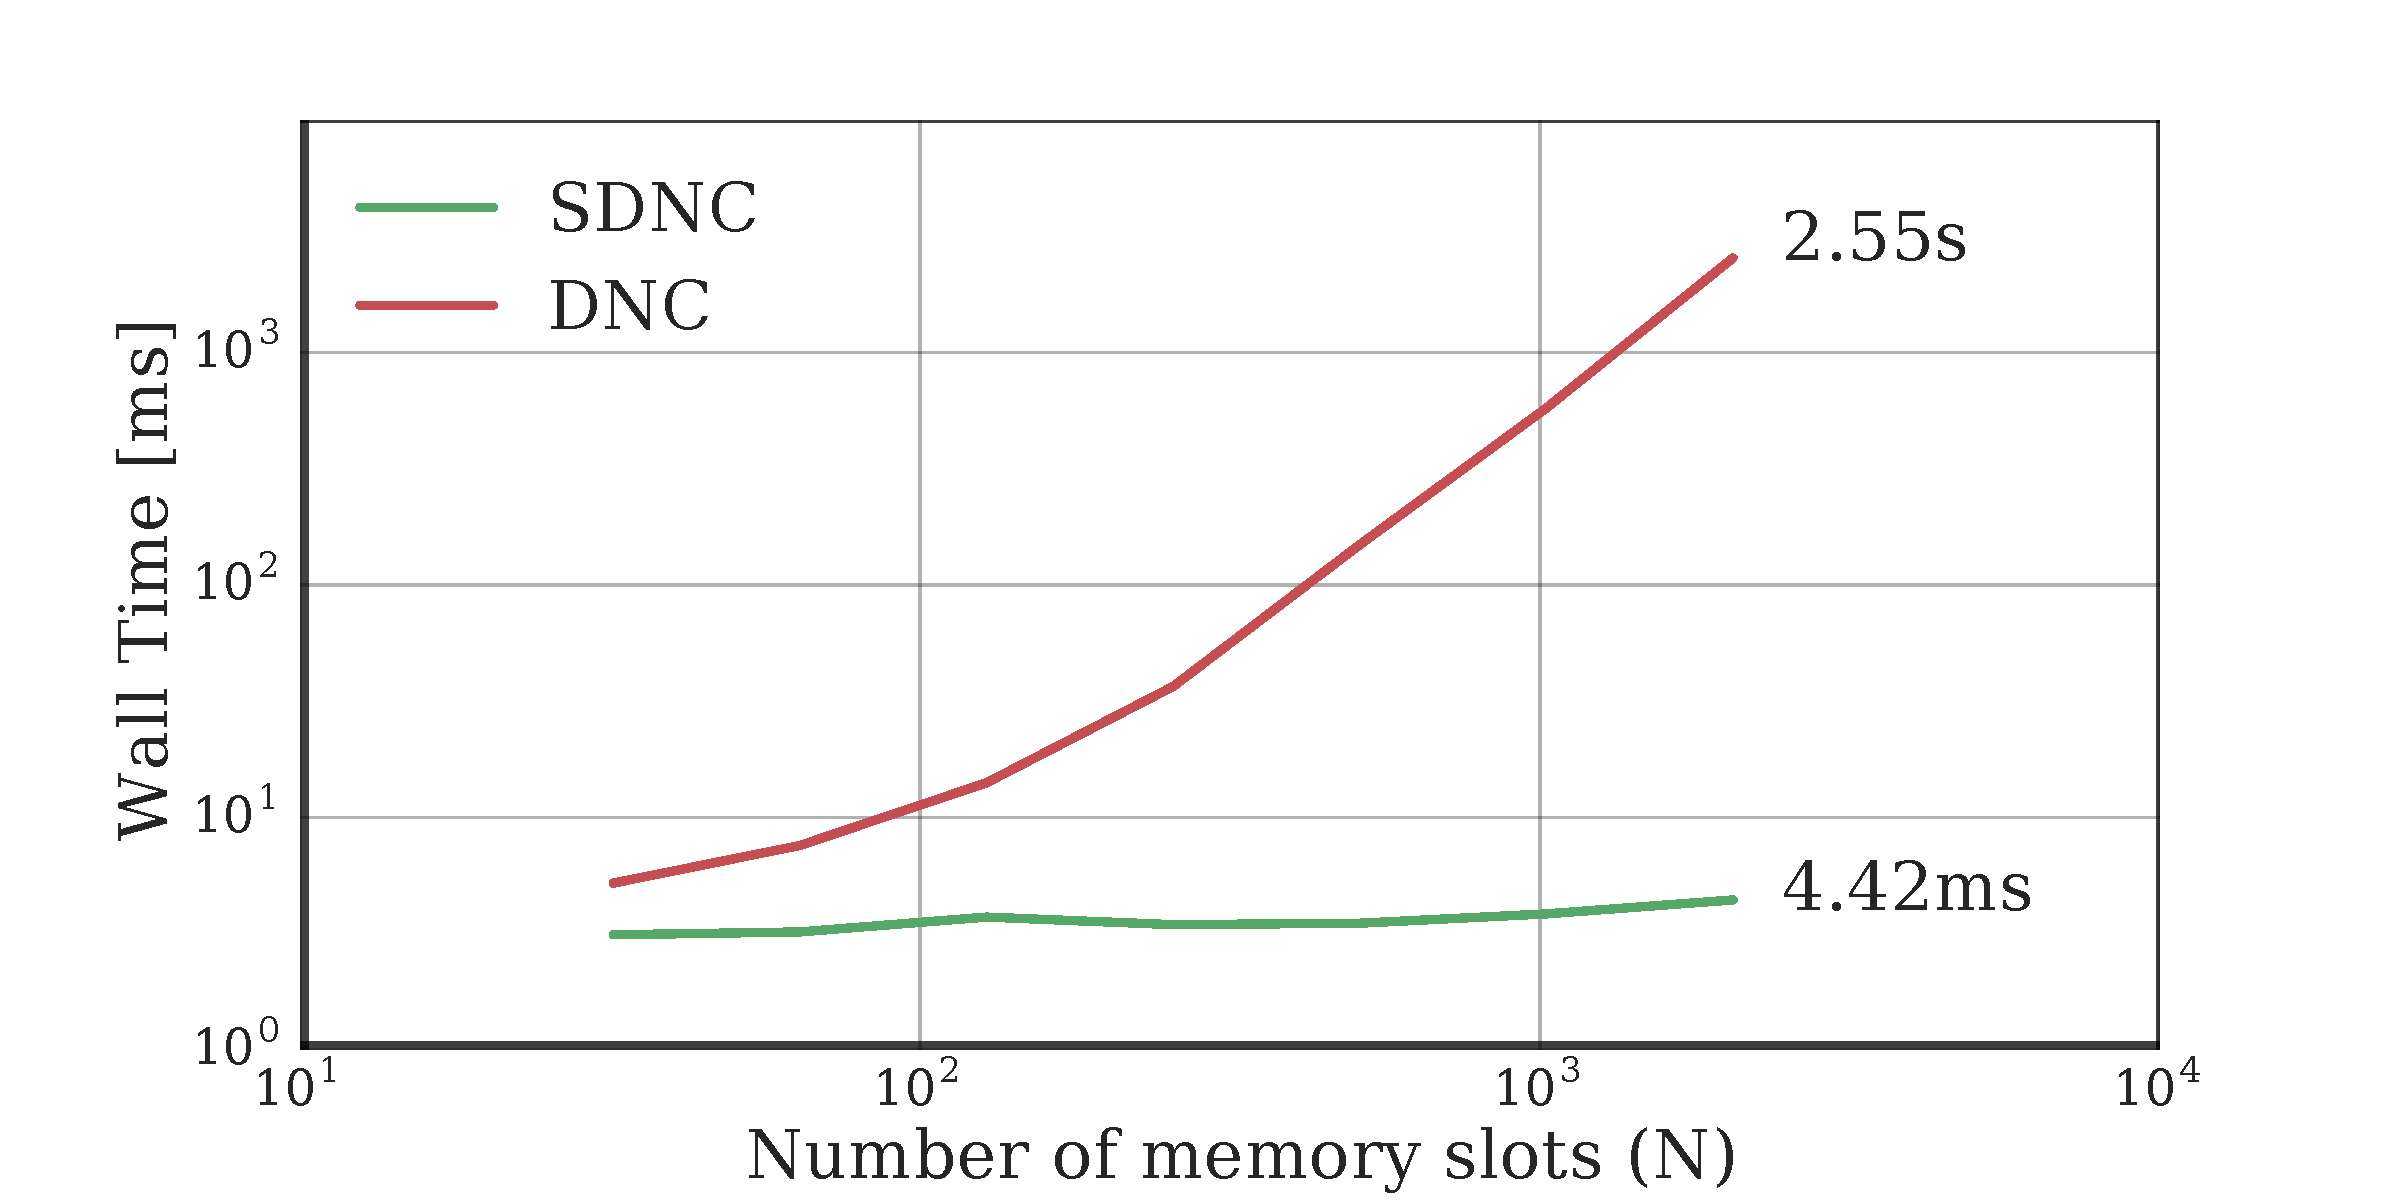
\includegraphics[height=3.4cm]{DNC_speed.pdf}
    \caption{ \label{sf:dnc_speed}}
    \end{subfigure}
    %
    % Memory
    \begin{subfigure}{0.47\textwidth}
    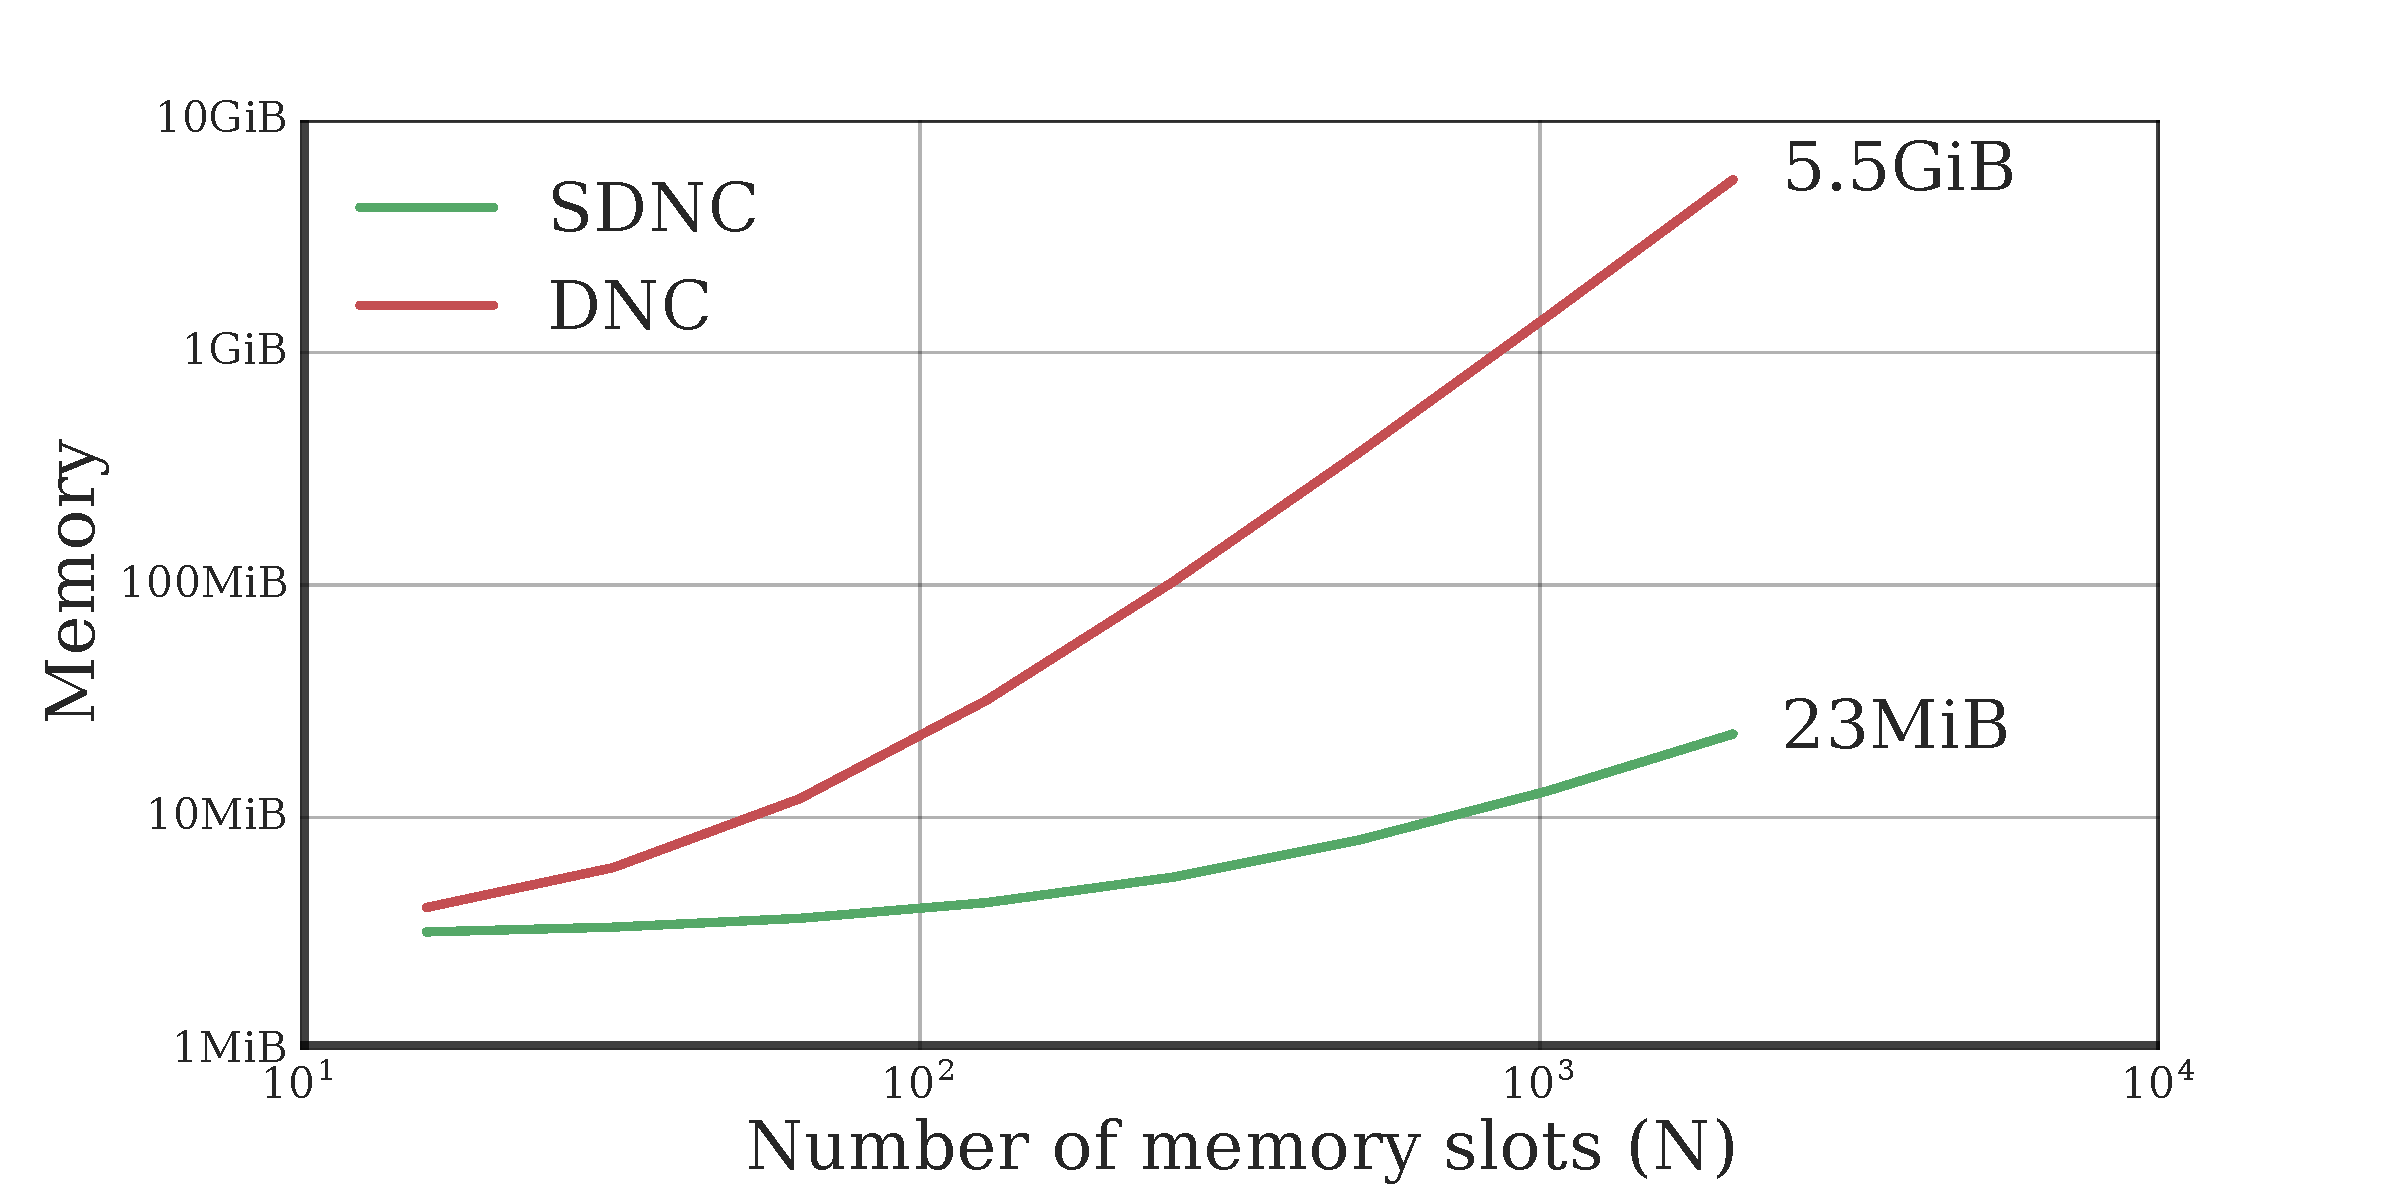
\includegraphics[height=3.4cm]{DNC_memory.pdf}
    \caption{ \label{sf:dnc_memory}}
    \end{subfigure}
    %
    \caption{Performance benchmarks between the DNC and SDNC for small to medium memory sizes. Here the SDNC uses a linear KNN. \textbf{(\subref{sf:dnc_speed})} Wall-clock time of a single forward and backward pass.
    \textbf{(\subref{sf:dnc_memory})} Total memory usage (including initialization) when trained over sequence of $10$ time steps.
    % When the memory contains 64,000 words the NTM consumes $\SI{29}{GiB}$ whereas SAM consumes only $\SI{7.8}{MiB}$, a compression ratio of $3700$.
    }
    \label{fig:dnc_perf_benchmarks}
\end{figure*}

In order to compare the models on an interesting task we ran the DNC and SDNC on the Babi task (this task is described more fully in the main text). The results are described in Supplementary \ref{sec:babi} and demonstrate the SDNC is capable of learning competitively. In particular, it achieves the best report result on the Babi task.


\section{Benchmarking details}
\label{sec:benchmarking}

Each model contained an LSTM controller with 100 hidden units, an external memory containing $N$ slots of memory, with word size $32$ and $4$ access heads. For speed benchmarks, a minibatch size of $8$ was used to ensure fair comparison - as many dense operations (e.g. matrix multiplication) can be batched efficiently. For memory benchmarks, the minibatch size was set to $1$.

We used Torch7 \cite{collobert2011torch7} to implement SAM, DAM, NTM, DNC and SDNC. Eigen v3 \cite{guennebaud2010eigen} was used for the fast sparse tensor operations, using the provided CSC and CSR formats. All benchmarks were run on a Linux desktop running Ubuntu 14.04.1 with 32GiB of RAM and an Intel Xeon E5-1650 3.20GHz processor with power scaling disabled.

\section{Generalization on associative recall}

\begin{figure}[h!]
    \centering
%    % From https://colab.corp.google.com/v2/notebook#fileId=0B3o-wCQ_1oEwYzhZQ3VKWFpHOGM&scrollTo=n_rVszHILw67
    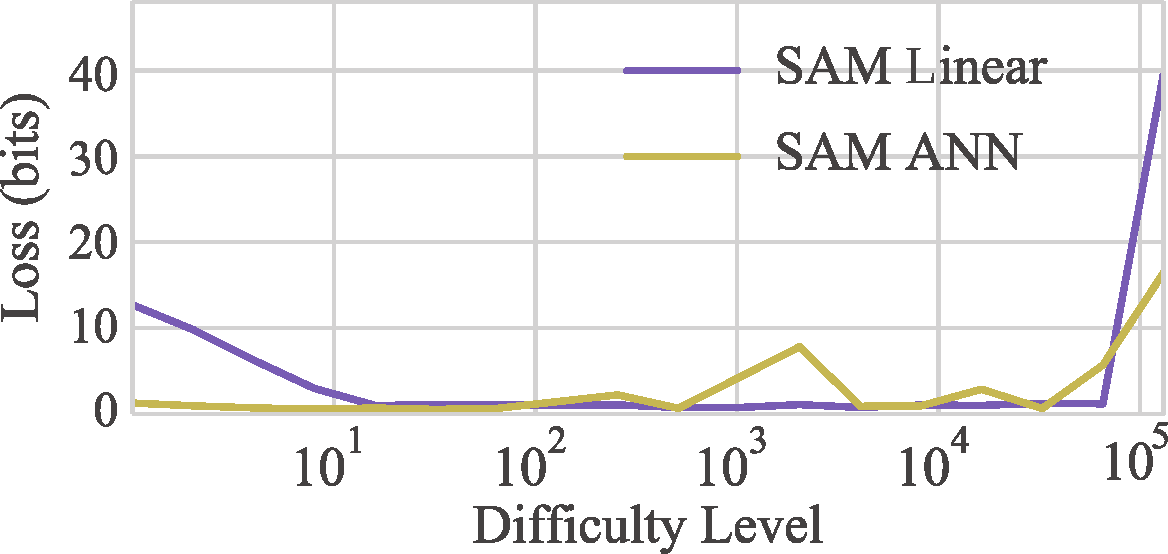
\includegraphics[width=0.6\linewidth]{extrapolation3throughpsb_cz}
    \caption{We tested the generalization of SAM on the associative recall task. We train each model up to a difficulty level, which corresponds to the task's sequence length, of $10,000$, and evaluate on longer sequences. The SAM models (with and without ANN) are able to perform much better than chance (48 bits) on sequences of length $200,000$.
    }
    \label{fig:extrapolation}
\end{figure}

\section{Babi results}
\label{sec:babi}

See the main text for a description of the Babi task and its relevance. Here we report the best and mean results for all of the models on this task.

The task was encoded using straightforward 1-hot word encodings for both the input and output. We trained a single model on all of the tasks, and used the 10,000 examples per task version of the training set (a small subset of which we used as a validation set for selecting the best run and hyperparameters). Previous work has reported best results (Supplementary table \ref{tab:babi:best}), which with only 15 runs is a noisy comparison, so we additionally report the mean and variance for all runs with the best selected hyperparameters (Supplementary table \ref{tab:babi:mean}).

\begin{landscape}

\begin{table}[]
    \centering
    \begin{tabular}{l|c|c|c|c|c|c|c|c}

% Table autogenerated from run 43.
% https://colab.corp.google.com/v2/notebook#fileId=0B3o-wCQ_1oEwSUpBSm1vWkxZc28&scrollTo=pdZNoSuGlS48
 & LSTM & DNC & SDNC & DAM & SAM & NTM & MN S & MN U \\
\hline
 1:    1 supporting fact  & $ 28.8$ & $  0.0$ & $  0.0$ & $  0.0$ & $  0.0$ & $ 16.4$ & $  0.0$ & $  0.0$ \\
 2:   2 supporting facts  & $ 57.3$ & $  3.2$ & $  0.6$ & $  0.2$ & $  0.2$ & $ 56.3$ & $  0.0$ & $  1.0$ \\
 3:   3 supporting facts  & $ 53.7$ & $  9.5$ & $  0.7$ & $  1.3$ & $  0.5$ & $ 49.0$ & $  0.0$ & $  6.8$ \\
 4: 2 argument relations  & $  0.7$ & $  0.0$ & $  0.0$ & $  0.0$ & $  0.0$ & $  0.0$ & $  0.0$ & $  0.0$ \\
 5: 3 argument relations  & $  3.5$ & $  1.7$ & $  0.3$ & $  0.4$ & $  0.7$ & $  2.5$ & $  0.3$ & $  6.1$ \\
 6:     yes/no questions  & $ 17.6$ & $  0.0$ & $  0.0$ & $  0.0$ & $  0.0$ & $  9.6$ & $  0.0$ & $  0.1$ \\
 7:             counting  & $ 18.5$ & $  5.3$ & $  0.2$ & $  0.4$ & $  1.9$ & $ 12.0$ & $  3.3$ & $  6.6$ \\
 8:           lists/sets  & $ 20.9$ & $  2.0$ & $  0.2$ & $  0.0$ & $  0.4$ & $  6.5$ & $  1.0$ & $  2.7$ \\
 9:      simple negation  & $ 18.2$ & $  0.1$ & $  0.0$ & $  0.0$ & $  0.1$ & $  7.0$ & $  0.0$ & $  0.0$ \\
10: indefinite knowledge  & $ 34.0$ & $  0.6$ & $  0.2$ & $  0.0$ & $  0.2$ & $  7.6$ & $  0.0$ & $  0.5$ \\
11:    basic coreference  & $  9.0$ & $  0.0$ & $  0.0$ & $  0.0$ & $  0.0$ & $  2.5$ & $  0.0$ & $  0.0$ \\
12:          conjunction  & $  5.5$ & $  0.1$ & $  0.1$ & $  0.0$ & $  0.1$ & $  4.6$ & $  0.0$ & $  0.1$ \\
13: compound coreference  & $  6.3$ & $  0.4$ & $  0.1$ & $  0.0$ & $  0.0$ & $  2.0$ & $  0.0$ & $  0.0$ \\
14:       time reasoning  & $ 56.1$ & $  0.2$ & $  0.1$ & $  3.8$ & $  4.3$ & $ 44.2$ & $  0.0$ & $  0.0$ \\
15:      basic deduction  & $ 49.3$ & $  0.1$ & $  0.0$ & $  0.0$ & $  0.0$ & $ 25.4$ & $  0.0$ & $  0.2$ \\
16:      basic induction  & $ 53.2$ & $ 51.9$ & $ 54.1$ & $ 52.8$ & $ 53.1$ & $ 52.2$ & $  0.0$ & $  0.2$ \\
17: positional reasoning  & $ 41.7$ & $ 21.7$ & $  0.3$ & $  6.0$ & $ 16.0$ & $ 39.7$ & $  0.0$ & $ 41.8$ \\
18:       size reasoning  & $  8.4$ & $  1.8$ & $  0.1$ & $  0.3$ & $  1.1$ & $  3.6$ & $ 24.6$ & $  8.0$ \\
19:         path finding  & $ 76.4$ & $  4.3$ & $  1.2$ & $  1.5$ & $  2.6$ & $  5.8$ & $  2.1$ & $ 75.7$ \\
20:  agent's motivations  & $  1.9$ & $  0.1$ & $  0.0$ & $  0.1$ & $  0.0$ & $  2.2$ & $ 31.9$ & $  0.0$ \\
\hline
Mean Error (\%)  & $ 28.0$ & $  5.2$ & $  2.9$ & $  3.3$ & $  4.1$ & $ 17.5$ & $  3.2$ & $  7.5$ \\
Failed tasks (err. > 5\%) & $   17$ & $    4$ & $    1$ & $    2$ & $    2$ & $   13$ & $    2$ & $    6$ \\
% End of autogenerated
    \end{tabular}
    \caption{Test results for the best run (chosen by validation set) on the Babi task. The model was trained and tested jointly on all tasks. All tasks received approximately equal training resources. Both SAM and DAM pass all but 2 of the tasks, without any supervision of their memory accesses. SDNC achieves the best reported result on this task with unsupervised memory access, solving all but 1 task.
    We've included comparison with memory networks, both with supervision of memories (MemNet S) and, more directly comparable with our approach, learning end-to-end (MemNets U). }
    \label{tab:babi:best}
\end{table}



\begin{table}[h]
    \centering
    \begin{tabular}{l|c|c|c|c|c|c}
% Table autogenerated from run 53.
% https://colab.corp.google.com/v2/notebook#fileId=0B3o-wCQ_1oEwSUpBSm1vWkxZc28&scrollTo=pdZNoSuGlS48
 & LSTM & DNC & SDNC & DAM & SAM & NTM \\
\hline
 1:    1 supporting fact  & $ 30.9 \pm   1.5$ & $  2.2 \pm   5.6$ & $  0.0 \pm   0.0$ & $  2.9 \pm  10.7$ & $  4.7 \pm  12.8$ & $ 31.5 \pm  15.3$ \\
 2:   2 supporting facts  & $ 57.4 \pm   1.2$ & $ 23.9 \pm  21.0$ & $  7.1 \pm  14.6$ & $ 12.1 \pm  19.3$ & $ 30.9 \pm  25.1$ & $ 57.0 \pm   1.3$ \\
 3:   3 supporting facts  & $ 53.0 \pm   1.4$ & $ 29.7 \pm  15.8$ & $  9.4 \pm  16.7$ & $ 15.3 \pm  17.4$ & $ 31.4 \pm  21.6$ & $ 49.4 \pm   1.3$ \\
 4: 2 argument relations  & $  0.7 \pm   0.4$ & $  0.1 \pm   0.1$ & $  0.1 \pm   0.1$ & $  0.1 \pm   0.1$ & $  0.2 \pm   0.2$ & $  0.4 \pm   0.3$ \\
 5: 3 argument relations  & $  4.9 \pm   0.9$ & $  1.3 \pm   0.3$ & $  0.9 \pm   0.3$ & $  1.0 \pm   0.4$ & $  1.0 \pm   0.5$ & $  2.7 \pm   1.2$ \\
 6:     yes/no questions  & $ 18.8 \pm   1.0$ & $  2.8 \pm   5.0$ & $  0.1 \pm   0.2$ & $  1.9 \pm   5.3$ & $  3.9 \pm   6.7$ & $ 18.6 \pm   2.7$ \\
 7:             counting  & $ 18.2 \pm   1.1$ & $  7.3 \pm   5.9$ & $  1.6 \pm   0.9$ & $  4.5 \pm   6.1$ & $  7.3 \pm   6.6$ & $ 18.7 \pm   3.2$ \\
 8:           lists/sets  & $ 20.9 \pm   1.4$ & $  4.0 \pm   4.1$ & $  0.5 \pm   0.4$ & $  2.7 \pm   5.4$ & $  3.6 \pm   6.2$ & $ 18.5 \pm   5.9$ \\
 9:      simple negation  & $ 19.4 \pm   1.5$ & $  3.0 \pm   5.2$ & $  0.0 \pm   0.1$ & $  2.1 \pm   5.5$ & $  3.8 \pm   6.7$ & $ 17.6 \pm   3.4$ \\
10: indefinite knowledge  & $ 33.0 \pm   1.6$ & $  3.2 \pm   5.9$ & $  0.3 \pm   0.2$ & $  3.4 \pm   8.1$ & $  5.7 \pm   9.2$ & $ 25.6 \pm   6.9$ \\
11:    basic coreference  & $ 15.9 \pm   3.3$ & $  0.9 \pm   3.0$ & $  0.0 \pm   0.0$ & $  1.5 \pm   5.5$ & $  2.6 \pm   7.9$ & $ 15.2 \pm   9.4$ \\
12:          conjunction  & $  7.0 \pm   1.3$ & $  1.5 \pm   1.6$ & $  0.2 \pm   0.3$ & $  1.8 \pm   6.4$ & $  2.9 \pm   7.9$ & $ 14.7 \pm   8.9$ \\
13: compound coreference  & $  9.1 \pm   1.4$ & $  1.5 \pm   2.5$ & $  0.1 \pm   0.1$ & $  0.6 \pm   2.2$ & $  1.3 \pm   2.4$ & $  6.8 \pm   3.3$ \\
14:       time reasoning  & $ 57.0 \pm   1.6$ & $ 10.6 \pm   9.4$ & $  5.6 \pm   2.9$ & $ 11.5 \pm  15.0$ & $ 15.0 \pm  12.6$ & $ 52.6 \pm   5.1$ \\
15:      basic deduction  & $ 48.1 \pm   1.3$ & $ 31.3 \pm  15.6$ & $  3.6 \pm  10.3$ & $ 17.2 \pm  19.7$ & $  5.5 \pm  13.8$ & $ 42.0 \pm   6.9$ \\
16:      basic induction  & $ 53.8 \pm   1.4$ & $ 54.0 \pm   1.9$ & $ 53.0 \pm   1.3$ & $ 53.8 \pm   1.0$ & $ 53.6 \pm   1.2$ & $ 53.8 \pm   2.1$ \\
17: positional reasoning  & $ 40.8 \pm   1.8$ & $ 27.7 \pm   9.4$ & $ 12.4 \pm   5.9$ & $ 16.9 \pm  10.3$ & $ 20.4 \pm   8.6$ & $ 40.1 \pm   1.3$ \\
18:       size reasoning  & $  7.3 \pm   1.9$ & $  3.5 \pm   1.5$ & $  1.6 \pm   1.1$ & $  1.8 \pm   1.7$ & $  3.0 \pm   1.8$ & $  5.0 \pm   1.2$ \\
19:         path finding  & $ 74.4 \pm   1.3$ & $ 44.9 \pm  29.0$ & $ 30.8 \pm  24.2$ & $ 23.0 \pm  25.4$ & $ 33.7 \pm  27.8$ & $ 60.8 \pm  24.6$ \\
20:  agent's motivations  & $  1.7 \pm   0.4$ & $  0.1 \pm   0.2$ & $  0.0 \pm   0.0$ & $  0.1 \pm   0.5$ & $  0.0 \pm   0.0$ & $  2.0 \pm   0.3$ \\
\hline
Mean Error (\%)  &
$ 28.7 \pm  0.5$ & $ 12.8 \pm  4.7$ & $  6.4 \pm  2.5$ & $  8.7 \pm  6.4$ & $ 11.5 \pm  5.9$ & $ 26.6 \pm  3.7$ \\
%$ 28.6 $ & $ 12.7 $ & $ 6.4 $ & $ 8.71 $ & $ 11.5 $ & $ 26.6 $ \\
Failed tasks (err. > 5\%) & $ 17.1 \pm  0.8$ & $  8.2 \pm  2.5$ & $  4.1 \pm  1.6$ & $  5.4 \pm  3.4$ & $  7.1 \pm  3.4$ & $ 15.5 \pm  1.7$ \\% End of autogenerated
    \end{tabular}
    \caption{Mean and variance of test errors for the best set of hyperparameters (chosen according the validation set). Statistics are generated from 15 runs.}
    \label{tab:babi:mean}
\end{table}

\end{landscape}

\end{document}
